\section{Implementacja rozmytych algorytmów PID i DMC}
\label{projekt:zad5}


W tym samym programie zaimplementowac i omówic rozmyty algorytm PID i rozmyty
algorytm DMC w najprostszej wersji analitycznej. Uzasadnic wybór zmiennej,
na podstawie której dokonywane jest rozmywanie. Uzasadnic wybór i kształt funkcji
przynaleznosci.

%\begin{figure}[H] 
%    \centering
%    % This file was created by matlab2tikz.
%
\definecolor{mycolor1}{rgb}{0.00000,0.44700,0.74100}%
%
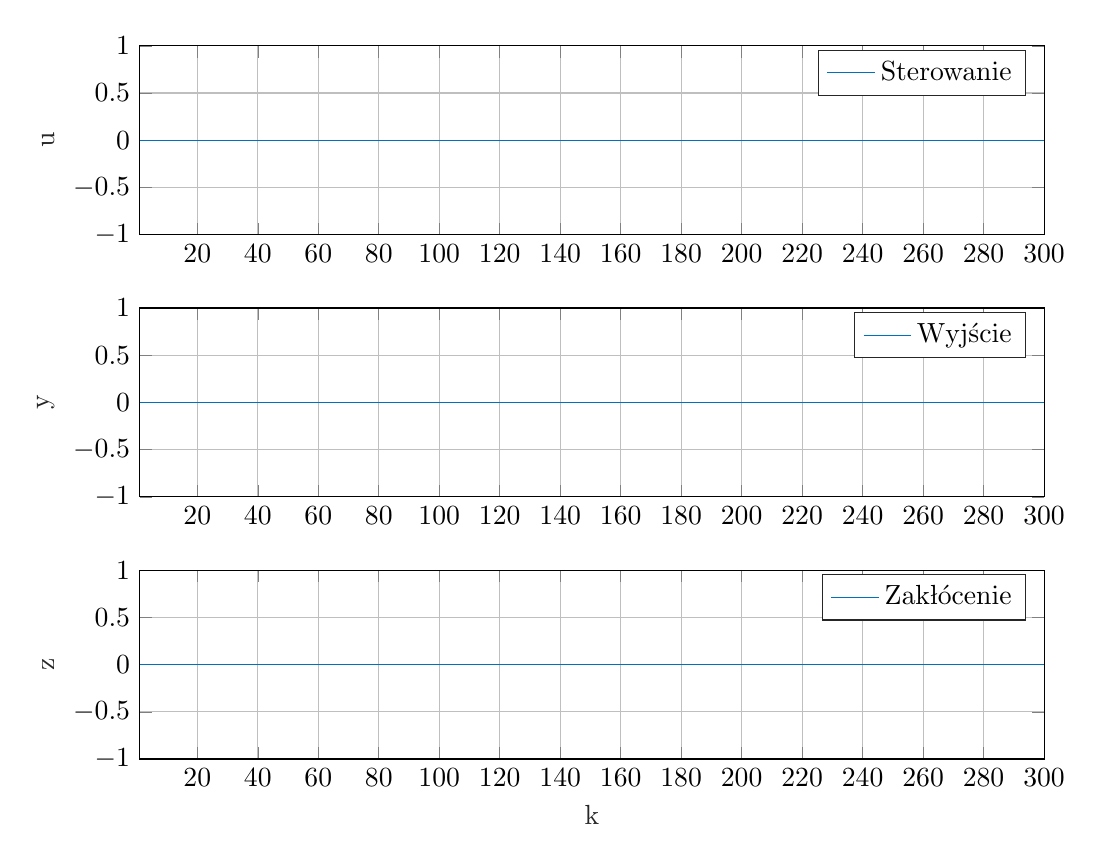
\begin{tikzpicture}

\begin{axis}[%
width=4.521in,
height=0.944in,
at={(0.758in,3.103in)},
scale only axis,
xmin=1,
xmax=300,
ymin=-1,
ymax=1,
ylabel style={font=\color{white!15!black}},
ylabel={u},
axis background/.style={fill=white},
xmajorgrids,
ymajorgrids,
legend style={legend cell align=left, align=left, draw=white!15!black}
]
\addplot [color=mycolor1]
  table[row sep=crcr]{%
1	0\\
2	0\\
3	0\\
4	0\\
5	0\\
6	0\\
7	0\\
8	0\\
9	0\\
10	0\\
11	0\\
12	0\\
13	0\\
14	0\\
15	0\\
16	0\\
17	0\\
18	0\\
19	0\\
20	0\\
21	0\\
22	0\\
23	0\\
24	0\\
25	0\\
26	0\\
27	0\\
28	0\\
29	0\\
30	0\\
31	0\\
32	0\\
33	0\\
34	0\\
35	0\\
36	0\\
37	0\\
38	0\\
39	0\\
40	0\\
41	0\\
42	0\\
43	0\\
44	0\\
45	0\\
46	0\\
47	0\\
48	0\\
49	0\\
50	0\\
51	0\\
52	0\\
53	0\\
54	0\\
55	0\\
56	0\\
57	0\\
58	0\\
59	0\\
60	0\\
61	0\\
62	0\\
63	0\\
64	0\\
65	0\\
66	0\\
67	0\\
68	0\\
69	0\\
70	0\\
71	0\\
72	0\\
73	0\\
74	0\\
75	0\\
76	0\\
77	0\\
78	0\\
79	0\\
80	0\\
81	0\\
82	0\\
83	0\\
84	0\\
85	0\\
86	0\\
87	0\\
88	0\\
89	0\\
90	0\\
91	0\\
92	0\\
93	0\\
94	0\\
95	0\\
96	0\\
97	0\\
98	0\\
99	0\\
100	0\\
101	0\\
102	0\\
103	0\\
104	0\\
105	0\\
106	0\\
107	0\\
108	0\\
109	0\\
110	0\\
111	0\\
112	0\\
113	0\\
114	0\\
115	0\\
116	0\\
117	0\\
118	0\\
119	0\\
120	0\\
121	0\\
122	0\\
123	0\\
124	0\\
125	0\\
126	0\\
127	0\\
128	0\\
129	0\\
130	0\\
131	0\\
132	0\\
133	0\\
134	0\\
135	0\\
136	0\\
137	0\\
138	0\\
139	0\\
140	0\\
141	0\\
142	0\\
143	0\\
144	0\\
145	0\\
146	0\\
147	0\\
148	0\\
149	0\\
150	0\\
151	0\\
152	0\\
153	0\\
154	0\\
155	0\\
156	0\\
157	0\\
158	0\\
159	0\\
160	0\\
161	0\\
162	0\\
163	0\\
164	0\\
165	0\\
166	0\\
167	0\\
168	0\\
169	0\\
170	0\\
171	0\\
172	0\\
173	0\\
174	0\\
175	0\\
176	0\\
177	0\\
178	0\\
179	0\\
180	0\\
181	0\\
182	0\\
183	0\\
184	0\\
185	0\\
186	0\\
187	0\\
188	0\\
189	0\\
190	0\\
191	0\\
192	0\\
193	0\\
194	0\\
195	0\\
196	0\\
197	0\\
198	0\\
199	0\\
200	0\\
201	0\\
202	0\\
203	0\\
204	0\\
205	0\\
206	0\\
207	0\\
208	0\\
209	0\\
210	0\\
211	0\\
212	0\\
213	0\\
214	0\\
215	0\\
216	0\\
217	0\\
218	0\\
219	0\\
220	0\\
221	0\\
222	0\\
223	0\\
224	0\\
225	0\\
226	0\\
227	0\\
228	0\\
229	0\\
230	0\\
231	0\\
232	0\\
233	0\\
234	0\\
235	0\\
236	0\\
237	0\\
238	0\\
239	0\\
240	0\\
241	0\\
242	0\\
243	0\\
244	0\\
245	0\\
246	0\\
247	0\\
248	0\\
249	0\\
250	0\\
251	0\\
252	0\\
253	0\\
254	0\\
255	0\\
256	0\\
257	0\\
258	0\\
259	0\\
260	0\\
261	0\\
262	0\\
263	0\\
264	0\\
265	0\\
266	0\\
267	0\\
268	0\\
269	0\\
270	0\\
271	0\\
272	0\\
273	0\\
274	0\\
275	0\\
276	0\\
277	0\\
278	0\\
279	0\\
280	0\\
281	0\\
282	0\\
283	0\\
284	0\\
285	0\\
286	0\\
287	0\\
288	0\\
289	0\\
290	0\\
291	0\\
292	0\\
293	0\\
294	0\\
295	0\\
296	0\\
297	0\\
298	0\\
299	0\\
300	0\\
};
\addlegendentry{Sterowanie}

\end{axis}

\begin{axis}[%
width=4.521in,
height=0.944in,
at={(0.758in,1.792in)},
scale only axis,
xmin=1,
xmax=300,
ymin=-1,
ymax=1,
ylabel style={font=\color{white!15!black}},
ylabel={y},
axis background/.style={fill=white},
xmajorgrids,
ymajorgrids,
legend style={legend cell align=left, align=left, draw=white!15!black}
]
\addplot [color=mycolor1]
  table[row sep=crcr]{%
1	0\\
2	0\\
3	0\\
4	0\\
5	0\\
6	0\\
7	0\\
8	0\\
9	0\\
10	0\\
11	0\\
12	0\\
13	0\\
14	0\\
15	0\\
16	0\\
17	0\\
18	0\\
19	0\\
20	0\\
21	0\\
22	0\\
23	0\\
24	0\\
25	0\\
26	0\\
27	0\\
28	0\\
29	0\\
30	0\\
31	0\\
32	0\\
33	0\\
34	0\\
35	0\\
36	0\\
37	0\\
38	0\\
39	0\\
40	0\\
41	0\\
42	0\\
43	0\\
44	0\\
45	0\\
46	0\\
47	0\\
48	0\\
49	0\\
50	0\\
51	0\\
52	0\\
53	0\\
54	0\\
55	0\\
56	0\\
57	0\\
58	0\\
59	0\\
60	0\\
61	0\\
62	0\\
63	0\\
64	0\\
65	0\\
66	0\\
67	0\\
68	0\\
69	0\\
70	0\\
71	0\\
72	0\\
73	0\\
74	0\\
75	0\\
76	0\\
77	0\\
78	0\\
79	0\\
80	0\\
81	0\\
82	0\\
83	0\\
84	0\\
85	0\\
86	0\\
87	0\\
88	0\\
89	0\\
90	0\\
91	0\\
92	0\\
93	0\\
94	0\\
95	0\\
96	0\\
97	0\\
98	0\\
99	0\\
100	0\\
101	0\\
102	0\\
103	0\\
104	0\\
105	0\\
106	0\\
107	0\\
108	0\\
109	0\\
110	0\\
111	0\\
112	0\\
113	0\\
114	0\\
115	0\\
116	0\\
117	0\\
118	0\\
119	0\\
120	0\\
121	0\\
122	0\\
123	0\\
124	0\\
125	0\\
126	0\\
127	0\\
128	0\\
129	0\\
130	0\\
131	0\\
132	0\\
133	0\\
134	0\\
135	0\\
136	0\\
137	0\\
138	0\\
139	0\\
140	0\\
141	0\\
142	0\\
143	0\\
144	0\\
145	0\\
146	0\\
147	0\\
148	0\\
149	0\\
150	0\\
151	0\\
152	0\\
153	0\\
154	0\\
155	0\\
156	0\\
157	0\\
158	0\\
159	0\\
160	0\\
161	0\\
162	0\\
163	0\\
164	0\\
165	0\\
166	0\\
167	0\\
168	0\\
169	0\\
170	0\\
171	0\\
172	0\\
173	0\\
174	0\\
175	0\\
176	0\\
177	0\\
178	0\\
179	0\\
180	0\\
181	0\\
182	0\\
183	0\\
184	0\\
185	0\\
186	0\\
187	0\\
188	0\\
189	0\\
190	0\\
191	0\\
192	0\\
193	0\\
194	0\\
195	0\\
196	0\\
197	0\\
198	0\\
199	0\\
200	0\\
201	0\\
202	0\\
203	0\\
204	0\\
205	0\\
206	0\\
207	0\\
208	0\\
209	0\\
210	0\\
211	0\\
212	0\\
213	0\\
214	0\\
215	0\\
216	0\\
217	0\\
218	0\\
219	0\\
220	0\\
221	0\\
222	0\\
223	0\\
224	0\\
225	0\\
226	0\\
227	0\\
228	0\\
229	0\\
230	0\\
231	0\\
232	0\\
233	0\\
234	0\\
235	0\\
236	0\\
237	0\\
238	0\\
239	0\\
240	0\\
241	0\\
242	0\\
243	0\\
244	0\\
245	0\\
246	0\\
247	0\\
248	0\\
249	0\\
250	0\\
251	0\\
252	0\\
253	0\\
254	0\\
255	0\\
256	0\\
257	0\\
258	0\\
259	0\\
260	0\\
261	0\\
262	0\\
263	0\\
264	0\\
265	0\\
266	0\\
267	0\\
268	0\\
269	0\\
270	0\\
271	0\\
272	0\\
273	0\\
274	0\\
275	0\\
276	0\\
277	0\\
278	0\\
279	0\\
280	0\\
281	0\\
282	0\\
283	0\\
284	0\\
285	0\\
286	0\\
287	0\\
288	0\\
289	0\\
290	0\\
291	0\\
292	0\\
293	0\\
294	0\\
295	0\\
296	0\\
297	0\\
298	0\\
299	0\\
300	0\\
};
\addlegendentry{Wyjście}

\end{axis}

\begin{axis}[%
width=4.521in,
height=0.944in,
at={(0.758in,0.481in)},
scale only axis,
xmin=1,
xmax=300,
xlabel style={font=\color{white!15!black}},
xlabel={k},
ymin=-1,
ymax=1,
ylabel style={font=\color{white!15!black}},
ylabel={z},
axis background/.style={fill=white},
xmajorgrids,
ymajorgrids,
legend style={legend cell align=left, align=left, draw=white!15!black}
]
\addplot [color=mycolor1]
  table[row sep=crcr]{%
1	0\\
2	0\\
3	0\\
4	0\\
5	0\\
6	0\\
7	0\\
8	0\\
9	0\\
10	0\\
11	0\\
12	0\\
13	0\\
14	0\\
15	0\\
16	0\\
17	0\\
18	0\\
19	0\\
20	0\\
21	0\\
22	0\\
23	0\\
24	0\\
25	0\\
26	0\\
27	0\\
28	0\\
29	0\\
30	0\\
31	0\\
32	0\\
33	0\\
34	0\\
35	0\\
36	0\\
37	0\\
38	0\\
39	0\\
40	0\\
41	0\\
42	0\\
43	0\\
44	0\\
45	0\\
46	0\\
47	0\\
48	0\\
49	0\\
50	0\\
51	0\\
52	0\\
53	0\\
54	0\\
55	0\\
56	0\\
57	0\\
58	0\\
59	0\\
60	0\\
61	0\\
62	0\\
63	0\\
64	0\\
65	0\\
66	0\\
67	0\\
68	0\\
69	0\\
70	0\\
71	0\\
72	0\\
73	0\\
74	0\\
75	0\\
76	0\\
77	0\\
78	0\\
79	0\\
80	0\\
81	0\\
82	0\\
83	0\\
84	0\\
85	0\\
86	0\\
87	0\\
88	0\\
89	0\\
90	0\\
91	0\\
92	0\\
93	0\\
94	0\\
95	0\\
96	0\\
97	0\\
98	0\\
99	0\\
100	0\\
101	0\\
102	0\\
103	0\\
104	0\\
105	0\\
106	0\\
107	0\\
108	0\\
109	0\\
110	0\\
111	0\\
112	0\\
113	0\\
114	0\\
115	0\\
116	0\\
117	0\\
118	0\\
119	0\\
120	0\\
121	0\\
122	0\\
123	0\\
124	0\\
125	0\\
126	0\\
127	0\\
128	0\\
129	0\\
130	0\\
131	0\\
132	0\\
133	0\\
134	0\\
135	0\\
136	0\\
137	0\\
138	0\\
139	0\\
140	0\\
141	0\\
142	0\\
143	0\\
144	0\\
145	0\\
146	0\\
147	0\\
148	0\\
149	0\\
150	0\\
151	0\\
152	0\\
153	0\\
154	0\\
155	0\\
156	0\\
157	0\\
158	0\\
159	0\\
160	0\\
161	0\\
162	0\\
163	0\\
164	0\\
165	0\\
166	0\\
167	0\\
168	0\\
169	0\\
170	0\\
171	0\\
172	0\\
173	0\\
174	0\\
175	0\\
176	0\\
177	0\\
178	0\\
179	0\\
180	0\\
181	0\\
182	0\\
183	0\\
184	0\\
185	0\\
186	0\\
187	0\\
188	0\\
189	0\\
190	0\\
191	0\\
192	0\\
193	0\\
194	0\\
195	0\\
196	0\\
197	0\\
198	0\\
199	0\\
200	0\\
201	0\\
202	0\\
203	0\\
204	0\\
205	0\\
206	0\\
207	0\\
208	0\\
209	0\\
210	0\\
211	0\\
212	0\\
213	0\\
214	0\\
215	0\\
216	0\\
217	0\\
218	0\\
219	0\\
220	0\\
221	0\\
222	0\\
223	0\\
224	0\\
225	0\\
226	0\\
227	0\\
228	0\\
229	0\\
230	0\\
231	0\\
232	0\\
233	0\\
234	0\\
235	0\\
236	0\\
237	0\\
238	0\\
239	0\\
240	0\\
241	0\\
242	0\\
243	0\\
244	0\\
245	0\\
246	0\\
247	0\\
248	0\\
249	0\\
250	0\\
251	0\\
252	0\\
253	0\\
254	0\\
255	0\\
256	0\\
257	0\\
258	0\\
259	0\\
260	0\\
261	0\\
262	0\\
263	0\\
264	0\\
265	0\\
266	0\\
267	0\\
268	0\\
269	0\\
270	0\\
271	0\\
272	0\\
273	0\\
274	0\\
275	0\\
276	0\\
277	0\\
278	0\\
279	0\\
280	0\\
281	0\\
282	0\\
283	0\\
284	0\\
285	0\\
286	0\\
287	0\\
288	0\\
289	0\\
290	0\\
291	0\\
292	0\\
293	0\\
294	0\\
295	0\\
296	0\\
297	0\\
298	0\\
299	0\\
300	0\\
};
\addlegendentry{Zakłócenie}

\end{axis}
\end{tikzpicture}%
%    \caption{Punkt pracy obiektu symulacji}
%    \label{projekt:zad1:figure:charstat_u_y_z}
%\end{figure}


\subsection{Funkcje przynależności}
\label{projekt:zad5:fuzzyFunctions}

\begin{figure}[H] 
    \centering
    % This file was created by matlab2tikz.
%
\definecolor{mycolor1}{rgb}{0.00000,0.44700,0.74100}%
\definecolor{mycolor2}{rgb}{0.85000,0.32500,0.09800}%
%
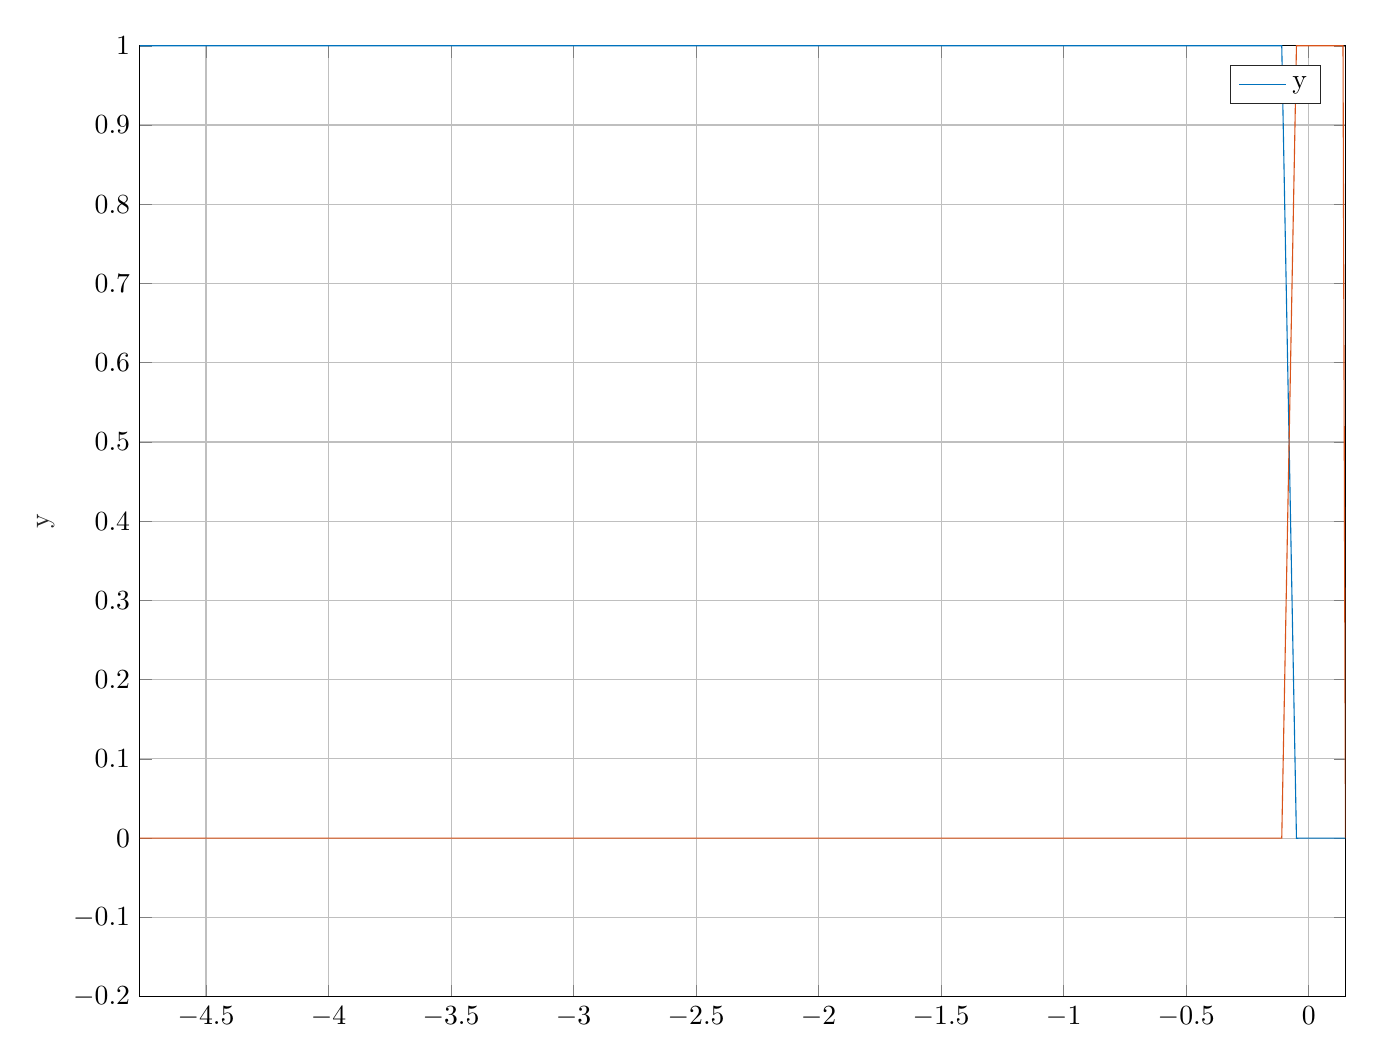
\begin{tikzpicture}

\begin{axis}[%
width=6.028in,
height=4.754in,
at={(1.011in,0.642in)},
scale only axis,
xmin=-4.77,
xmax=0.15,
ymin=-0.2,
ymax=1,
ylabel style={font=\color{white!15!black}},
ylabel={y},
axis background/.style={fill=white},
xmajorgrids,
ymajorgrids,
legend style={legend cell align=left, align=left, draw=white!15!black}
]
\addplot [color=mycolor1]
  table[row sep=crcr]{%
-4.77	1\\
-4.76	1\\
-4.75	1\\
-4.74	1\\
-4.73	1\\
-4.72	1\\
-4.71	1\\
-4.7	1\\
-4.69	1\\
-4.68	1\\
-4.67	1\\
-4.66	1\\
-4.65	1\\
-4.64	1\\
-4.63	1\\
-4.62	1\\
-4.61	1\\
-4.6	1\\
-4.59	1\\
-4.58	1\\
-4.57	1\\
-4.56	1\\
-4.55	1\\
-4.54	1\\
-4.53	1\\
-4.52	1\\
-4.51	1\\
-4.5	1\\
-4.49	1\\
-4.48	1\\
-4.47	1\\
-4.46	1\\
-4.45	1\\
-4.44	1\\
-4.43	1\\
-4.42	1\\
-4.41	1\\
-4.4	1\\
-4.39	1\\
-4.38	1\\
-4.37	1\\
-4.36	1\\
-4.35	1\\
-4.34	1\\
-4.33	1\\
-4.32	1\\
-4.31	1\\
-4.3	1\\
-4.29	1\\
-4.28	1\\
-4.27	1\\
-4.26	1\\
-4.25	1\\
-4.24	1\\
-4.23	1\\
-4.22	1\\
-4.21	1\\
-4.2	1\\
-4.19	1\\
-4.18	1\\
-4.17	1\\
-4.16	1\\
-4.15	1\\
-4.14	1\\
-4.13	1\\
-4.12	1\\
-4.11	1\\
-4.1	1\\
-4.09	1\\
-4.08	1\\
-4.07	1\\
-4.06	1\\
-4.05	1\\
-4.04	1\\
-4.03	1\\
-4.02	1\\
-4.01	1\\
-4	1\\
-3.99	1\\
-3.98	1\\
-3.97	1\\
-3.96	1\\
-3.95	1\\
-3.94	1\\
-3.93	1\\
-3.92	1\\
-3.91	1\\
-3.9	1\\
-3.89	1\\
-3.88	1\\
-3.87	1\\
-3.86	1\\
-3.85	1\\
-3.84	1\\
-3.83	1\\
-3.82	1\\
-3.81	1\\
-3.8	1\\
-3.79	1\\
-3.78	1\\
-3.77	1\\
-3.76	1\\
-3.75	1\\
-3.74	1\\
-3.73	1\\
-3.72	1\\
-3.71	1\\
-3.7	1\\
-3.69	1\\
-3.68	1\\
-3.67	1\\
-3.66	1\\
-3.65	1\\
-3.64	1\\
-3.63	1\\
-3.62	1\\
-3.61	1\\
-3.6	1\\
-3.59	1\\
-3.58	1\\
-3.57	1\\
-3.56	1\\
-3.55	1\\
-3.54	1\\
-3.53	1\\
-3.52	1\\
-3.51	1\\
-3.5	1\\
-3.49	1\\
-3.48	1\\
-3.47	1\\
-3.46	1\\
-3.45	1\\
-3.44	1\\
-3.43	1\\
-3.42	1\\
-3.41	1\\
-3.4	1\\
-3.39	1\\
-3.38	1\\
-3.37	1\\
-3.36	1\\
-3.35	1\\
-3.34	1\\
-3.33	1\\
-3.32	1\\
-3.31	1\\
-3.3	1\\
-3.29	1\\
-3.28	1\\
-3.27	1\\
-3.26	1\\
-3.25	1\\
-3.24	1\\
-3.23	1\\
-3.22	1\\
-3.21	1\\
-3.2	1\\
-3.19	1\\
-3.18	1\\
-3.17	1\\
-3.16	1\\
-3.15	1\\
-3.14	1\\
-3.13	1\\
-3.12	1\\
-3.11	1\\
-3.1	1\\
-3.09	1\\
-3.08	1\\
-3.07	1\\
-3.06	1\\
-3.05	1\\
-3.04	1\\
-3.03	1\\
-3.02	1\\
-3.01	1\\
-3	1\\
-2.99	1\\
-2.98	1\\
-2.97	1\\
-2.96	1\\
-2.95	1\\
-2.94	1\\
-2.93	1\\
-2.92	1\\
-2.91	1\\
-2.9	1\\
-2.89	1\\
-2.88	1\\
-2.87	1\\
-2.86	1\\
-2.85	1\\
-2.84	1\\
-2.83	1\\
-2.82	1\\
-2.81	1\\
-2.8	1\\
-2.79	1\\
-2.78	1\\
-2.77	1\\
-2.76	1\\
-2.75	1\\
-2.74	1\\
-2.73	1\\
-2.72	1\\
-2.71	1\\
-2.7	1\\
-2.69	1\\
-2.68	1\\
-2.67	1\\
-2.66	1\\
-2.65	1\\
-2.64	1\\
-2.63	1\\
-2.62	1\\
-2.61	1\\
-2.6	1\\
-2.59	1\\
-2.58	1\\
-2.57	1\\
-2.56	1\\
-2.55	1\\
-2.54	1\\
-2.53	1\\
-2.52	1\\
-2.51	1\\
-2.5	1\\
-2.49	1\\
-2.48	1\\
-2.47	1\\
-2.46	1\\
-2.45	1\\
-2.44	1\\
-2.43	1\\
-2.42	1\\
-2.41	1\\
-2.4	1\\
-2.39	1\\
-2.38	1\\
-2.37	1\\
-2.36	1\\
-2.35	1\\
-2.34	1\\
-2.33	1\\
-2.32	1\\
-2.31	1\\
-2.3	1\\
-2.29	1\\
-2.28	1\\
-2.27	1\\
-2.26	1\\
-2.25	1\\
-2.24	1\\
-2.23	1\\
-2.22	1\\
-2.21	1\\
-2.2	1\\
-2.19	1\\
-2.18	1\\
-2.17	1\\
-2.16	1\\
-2.15	1\\
-2.14	1\\
-2.13	1\\
-2.12	1\\
-2.11	1\\
-2.1	1\\
-2.09	1\\
-2.08	1\\
-2.07	1\\
-2.06	1\\
-2.05	1\\
-2.04	1\\
-2.03	1\\
-2.02	1\\
-2.01	1\\
-2	1\\
-1.99	1\\
-1.98	1\\
-1.97	1\\
-1.96	1\\
-1.95	1\\
-1.94	1\\
-1.93	1\\
-1.92	1\\
-1.91	1\\
-1.9	1\\
-1.89	1\\
-1.88	1\\
-1.87	1\\
-1.86	1\\
-1.85	1\\
-1.84	1\\
-1.83	1\\
-1.82	1\\
-1.81	1\\
-1.8	1\\
-1.79	1\\
-1.78	1\\
-1.77	1\\
-1.76	1\\
-1.75	1\\
-1.74	1\\
-1.73	1\\
-1.72	1\\
-1.71	1\\
-1.7	1\\
-1.69	1\\
-1.68	1\\
-1.67	1\\
-1.66	1\\
-1.65	1\\
-1.64	1\\
-1.63	1\\
-1.62	1\\
-1.61	1\\
-1.6	1\\
-1.59	1\\
-1.58	1\\
-1.57	1\\
-1.56	1\\
-1.55	1\\
-1.54	1\\
-1.53	1\\
-1.52	1\\
-1.51	1\\
-1.5	1\\
-1.49	1\\
-1.48	1\\
-1.47	1\\
-1.46	1\\
-1.45	1\\
-1.44	1\\
-1.43	1\\
-1.42	1\\
-1.41	1\\
-1.4	1\\
-1.39	1\\
-1.38	1\\
-1.37	1\\
-1.36	1\\
-1.35	1\\
-1.34	1\\
-1.33	1\\
-1.32	1\\
-1.31	1\\
-1.3	1\\
-1.29	1\\
-1.28	1\\
-1.27	1\\
-1.26	1\\
-1.25	1\\
-1.24	1\\
-1.23	1\\
-1.22	1\\
-1.21	1\\
-1.2	1\\
-1.19	1\\
-1.18	1\\
-1.17	1\\
-1.16	1\\
-1.15	1\\
-1.14	1\\
-1.13	1\\
-1.12	1\\
-1.11	1\\
-1.1	1\\
-1.09	1\\
-1.08	1\\
-1.07	1\\
-1.06	1\\
-1.05	1\\
-1.04	1\\
-1.03	1\\
-1.02	1\\
-1.01	1\\
-1	1\\
-0.99	1\\
-0.98	1\\
-0.97	1\\
-0.96	1\\
-0.95	1\\
-0.94	1\\
-0.93	1\\
-0.92	1\\
-0.91	1\\
-0.9	1\\
-0.89	1\\
-0.88	1\\
-0.87	1\\
-0.86	1\\
-0.85	1\\
-0.84	1\\
-0.83	1\\
-0.82	1\\
-0.81	1\\
-0.8	1\\
-0.79	1\\
-0.78	1\\
-0.77	1\\
-0.76	1\\
-0.75	1\\
-0.74	1\\
-0.73	1\\
-0.72	1\\
-0.71	1\\
-0.7	1\\
-0.69	1\\
-0.68	1\\
-0.67	1\\
-0.66	1\\
-0.65	1\\
-0.64	1\\
-0.63	1\\
-0.62	1\\
-0.61	1\\
-0.6	1\\
-0.59	1\\
-0.58	1\\
-0.57	1\\
-0.56	1\\
-0.55	1\\
-0.54	1\\
-0.53	1\\
-0.52	1\\
-0.51	1\\
-0.5	1\\
-0.49	1\\
-0.48	1\\
-0.47	1\\
-0.46	1\\
-0.45	1\\
-0.44	1\\
-0.43	1\\
-0.42	1\\
-0.41	1\\
-0.4	1\\
-0.39	1\\
-0.38	1\\
-0.37	1\\
-0.36	1\\
-0.35	1\\
-0.34	1\\
-0.33	1\\
-0.32	1\\
-0.31	1\\
-0.3	1\\
-0.29	1\\
-0.28	1\\
-0.27	1\\
-0.26	1\\
-0.25	1\\
-0.24	1\\
-0.23	1\\
-0.22	1\\
-0.21	1\\
-0.2	1\\
-0.19	1\\
-0.18	1\\
-0.17	1\\
-0.16	1\\
-0.15	1\\
-0.14	1\\
-0.13	1\\
-0.12	1\\
-0.11	1\\
-0.1	0.8333\\
-0.09	0.6666\\
-0.08	0.4999\\
-0.07	0.3332\\
-0.06	0.1665\\
-0.05	-0.0002\\
-0.04	0\\
-0.03	0\\
-0.02	0\\
-0.01	0\\
0	0\\
0.01	0\\
0.02	0\\
0.03	0\\
0.04	0\\
0.05	0\\
0.06	0\\
0.07	0\\
0.08	0\\
0.09	0\\
0.1	0\\
0.11	0\\
0.12	0\\
0.13	0\\
0.14	0\\
0.15	0\\
};
\addlegendentry{y}

\addplot [color=mycolor2, forget plot]
  table[row sep=crcr]{%
-4.77	0\\
-4.76	0\\
-4.75	0\\
-4.74	0\\
-4.73	0\\
-4.72	0\\
-4.71	0\\
-4.7	0\\
-4.69	0\\
-4.68	0\\
-4.67	0\\
-4.66	0\\
-4.65	0\\
-4.64	0\\
-4.63	0\\
-4.62	0\\
-4.61	0\\
-4.6	0\\
-4.59	0\\
-4.58	0\\
-4.57	0\\
-4.56	0\\
-4.55	0\\
-4.54	0\\
-4.53	0\\
-4.52	0\\
-4.51	0\\
-4.5	0\\
-4.49	0\\
-4.48	0\\
-4.47	0\\
-4.46	0\\
-4.45	0\\
-4.44	0\\
-4.43	0\\
-4.42	0\\
-4.41	0\\
-4.4	0\\
-4.39	0\\
-4.38	0\\
-4.37	0\\
-4.36	0\\
-4.35	0\\
-4.34	0\\
-4.33	0\\
-4.32	0\\
-4.31	0\\
-4.3	0\\
-4.29	0\\
-4.28	0\\
-4.27	0\\
-4.26	0\\
-4.25	0\\
-4.24	0\\
-4.23	0\\
-4.22	0\\
-4.21	0\\
-4.2	0\\
-4.19	0\\
-4.18	0\\
-4.17	0\\
-4.16	0\\
-4.15	0\\
-4.14	0\\
-4.13	0\\
-4.12	0\\
-4.11	0\\
-4.1	0\\
-4.09	0\\
-4.08	0\\
-4.07	0\\
-4.06	0\\
-4.05	0\\
-4.04	0\\
-4.03	0\\
-4.02	0\\
-4.01	0\\
-4	0\\
-3.99	0\\
-3.98	0\\
-3.97	0\\
-3.96	0\\
-3.95	0\\
-3.94	0\\
-3.93	0\\
-3.92	0\\
-3.91	0\\
-3.9	0\\
-3.89	0\\
-3.88	0\\
-3.87	0\\
-3.86	0\\
-3.85	0\\
-3.84	0\\
-3.83	0\\
-3.82	0\\
-3.81	0\\
-3.8	0\\
-3.79	0\\
-3.78	0\\
-3.77	0\\
-3.76	0\\
-3.75	0\\
-3.74	0\\
-3.73	0\\
-3.72	0\\
-3.71	0\\
-3.7	0\\
-3.69	0\\
-3.68	0\\
-3.67	0\\
-3.66	0\\
-3.65	0\\
-3.64	0\\
-3.63	0\\
-3.62	0\\
-3.61	0\\
-3.6	0\\
-3.59	0\\
-3.58	0\\
-3.57	0\\
-3.56	0\\
-3.55	0\\
-3.54	0\\
-3.53	0\\
-3.52	0\\
-3.51	0\\
-3.5	0\\
-3.49	0\\
-3.48	0\\
-3.47	0\\
-3.46	0\\
-3.45	0\\
-3.44	0\\
-3.43	0\\
-3.42	0\\
-3.41	0\\
-3.4	0\\
-3.39	0\\
-3.38	0\\
-3.37	0\\
-3.36	0\\
-3.35	0\\
-3.34	0\\
-3.33	0\\
-3.32	0\\
-3.31	0\\
-3.3	0\\
-3.29	0\\
-3.28	0\\
-3.27	0\\
-3.26	0\\
-3.25	0\\
-3.24	0\\
-3.23	0\\
-3.22	0\\
-3.21	0\\
-3.2	0\\
-3.19	0\\
-3.18	0\\
-3.17	0\\
-3.16	0\\
-3.15	0\\
-3.14	0\\
-3.13	0\\
-3.12	0\\
-3.11	0\\
-3.1	0\\
-3.09	0\\
-3.08	0\\
-3.07	0\\
-3.06	0\\
-3.05	0\\
-3.04	0\\
-3.03	0\\
-3.02	0\\
-3.01	0\\
-3	0\\
-2.99	0\\
-2.98	0\\
-2.97	0\\
-2.96	0\\
-2.95	0\\
-2.94	0\\
-2.93	0\\
-2.92	0\\
-2.91	0\\
-2.9	0\\
-2.89	0\\
-2.88	0\\
-2.87	0\\
-2.86	0\\
-2.85	0\\
-2.84	0\\
-2.83	0\\
-2.82	0\\
-2.81	0\\
-2.8	0\\
-2.79	0\\
-2.78	0\\
-2.77	0\\
-2.76	0\\
-2.75	0\\
-2.74	0\\
-2.73	0\\
-2.72	0\\
-2.71	0\\
-2.7	0\\
-2.69	0\\
-2.68	0\\
-2.67	0\\
-2.66	0\\
-2.65	0\\
-2.64	0\\
-2.63	0\\
-2.62	0\\
-2.61	0\\
-2.6	0\\
-2.59	0\\
-2.58	0\\
-2.57	0\\
-2.56	0\\
-2.55	0\\
-2.54	0\\
-2.53	0\\
-2.52	0\\
-2.51	0\\
-2.5	0\\
-2.49	0\\
-2.48	0\\
-2.47	0\\
-2.46	0\\
-2.45	0\\
-2.44	0\\
-2.43	0\\
-2.42	0\\
-2.41	0\\
-2.4	0\\
-2.39	0\\
-2.38	0\\
-2.37	0\\
-2.36	0\\
-2.35	0\\
-2.34	0\\
-2.33	0\\
-2.32	0\\
-2.31	0\\
-2.3	0\\
-2.29	0\\
-2.28	0\\
-2.27	0\\
-2.26	0\\
-2.25	0\\
-2.24	0\\
-2.23	0\\
-2.22	0\\
-2.21	0\\
-2.2	0\\
-2.19	0\\
-2.18	0\\
-2.17	0\\
-2.16	0\\
-2.15	0\\
-2.14	0\\
-2.13	0\\
-2.12	0\\
-2.11	0\\
-2.1	0\\
-2.09	0\\
-2.08	0\\
-2.07	0\\
-2.06	0\\
-2.05	0\\
-2.04	0\\
-2.03	0\\
-2.02	0\\
-2.01	0\\
-2	0\\
-1.99	0\\
-1.98	0\\
-1.97	0\\
-1.96	0\\
-1.95	0\\
-1.94	0\\
-1.93	0\\
-1.92	0\\
-1.91	0\\
-1.9	0\\
-1.89	0\\
-1.88	0\\
-1.87	0\\
-1.86	0\\
-1.85	0\\
-1.84	0\\
-1.83	0\\
-1.82	0\\
-1.81	0\\
-1.8	0\\
-1.79	0\\
-1.78	0\\
-1.77	0\\
-1.76	0\\
-1.75	0\\
-1.74	0\\
-1.73	0\\
-1.72	0\\
-1.71	0\\
-1.7	0\\
-1.69	0\\
-1.68	0\\
-1.67	0\\
-1.66	0\\
-1.65	0\\
-1.64	0\\
-1.63	0\\
-1.62	0\\
-1.61	0\\
-1.6	0\\
-1.59	0\\
-1.58	0\\
-1.57	0\\
-1.56	0\\
-1.55	0\\
-1.54	0\\
-1.53	0\\
-1.52	0\\
-1.51	0\\
-1.5	0\\
-1.49	0\\
-1.48	0\\
-1.47	0\\
-1.46	0\\
-1.45	0\\
-1.44	0\\
-1.43	0\\
-1.42	0\\
-1.41	0\\
-1.4	0\\
-1.39	0\\
-1.38	0\\
-1.37	0\\
-1.36	0\\
-1.35	0\\
-1.34	0\\
-1.33	0\\
-1.32	0\\
-1.31	0\\
-1.3	0\\
-1.29	0\\
-1.28	0\\
-1.27	0\\
-1.26	0\\
-1.25	0\\
-1.24	0\\
-1.23	0\\
-1.22	0\\
-1.21	0\\
-1.2	0\\
-1.19	0\\
-1.18	0\\
-1.17	0\\
-1.16	0\\
-1.15	0\\
-1.14	0\\
-1.13	0\\
-1.12	0\\
-1.11	0\\
-1.1	0\\
-1.09	0\\
-1.08	0\\
-1.07	0\\
-1.06	0\\
-1.05	0\\
-1.04	0\\
-1.03	0\\
-1.02	0\\
-1.01	0\\
-1	0\\
-0.99	0\\
-0.98	0\\
-0.97	0\\
-0.96	0\\
-0.95	0\\
-0.94	0\\
-0.93	0\\
-0.92	0\\
-0.91	0\\
-0.9	0\\
-0.89	0\\
-0.88	0\\
-0.87	0\\
-0.86	0\\
-0.85	0\\
-0.84	0\\
-0.83	0\\
-0.82	0\\
-0.81	0\\
-0.8	0\\
-0.79	0\\
-0.78	0\\
-0.77	0\\
-0.76	0\\
-0.75	0\\
-0.74	0\\
-0.73	0\\
-0.72	0\\
-0.71	0\\
-0.7	0\\
-0.69	0\\
-0.68	0\\
-0.67	0\\
-0.66	0\\
-0.65	0\\
-0.64	0\\
-0.63	0\\
-0.62	0\\
-0.61	0\\
-0.6	0\\
-0.59	0\\
-0.58	0\\
-0.57	0\\
-0.56	0\\
-0.55	0\\
-0.54	0\\
-0.53	0\\
-0.52	0\\
-0.51	0\\
-0.5	0\\
-0.49	0\\
-0.48	0\\
-0.47	0\\
-0.46	0\\
-0.45	0\\
-0.44	0\\
-0.43	0\\
-0.42	0\\
-0.41	0\\
-0.4	0\\
-0.39	0\\
-0.38	0\\
-0.37	0\\
-0.36	0\\
-0.35	0\\
-0.34	0\\
-0.33	0\\
-0.32	0\\
-0.31	0\\
-0.3	0\\
-0.29	0\\
-0.28	0\\
-0.27	0\\
-0.26	0\\
-0.25	0\\
-0.24	0\\
-0.23	0\\
-0.22	0\\
-0.21	0\\
-0.2	0\\
-0.19	0\\
-0.18	0\\
-0.17	0\\
-0.16	0\\
-0.15	0\\
-0.14	0\\
-0.13	0\\
-0.12	0\\
-0.11	-2.2204e-16\\
-0.1	0.1667\\
-0.09	0.3334\\
-0.08	0.5001\\
-0.07	0.6668\\
-0.06	0.8335\\
-0.05	1\\
-0.04	1\\
-0.03	1\\
-0.02	1\\
-0.01	1\\
0	1\\
0.01	1\\
0.02	1\\
0.03	1\\
0.04	1\\
0.05	1\\
0.06	1\\
0.07	1\\
0.08	1\\
0.09	1\\
0.1	1\\
0.11	1\\
0.12	1\\
0.13	1\\
0.14	1\\
0.15	0\\
};
\end{axis}
\end{tikzpicture}%
    \caption{Funkcje rozmycia dla 2 regulatorów lokalnych}
    \label{lab:zad4:fuzzyFunction:2:figure}
\end{figure}

\begin{figure}[H] 
    \centering
    % This file was created by matlab2tikz.
%
\definecolor{mycolor1}{rgb}{0.00000,0.44700,0.74100}%
\definecolor{mycolor2}{rgb}{0.85000,0.32500,0.09800}%
\definecolor{mycolor3}{rgb}{0.92900,0.69400,0.12500}%
%
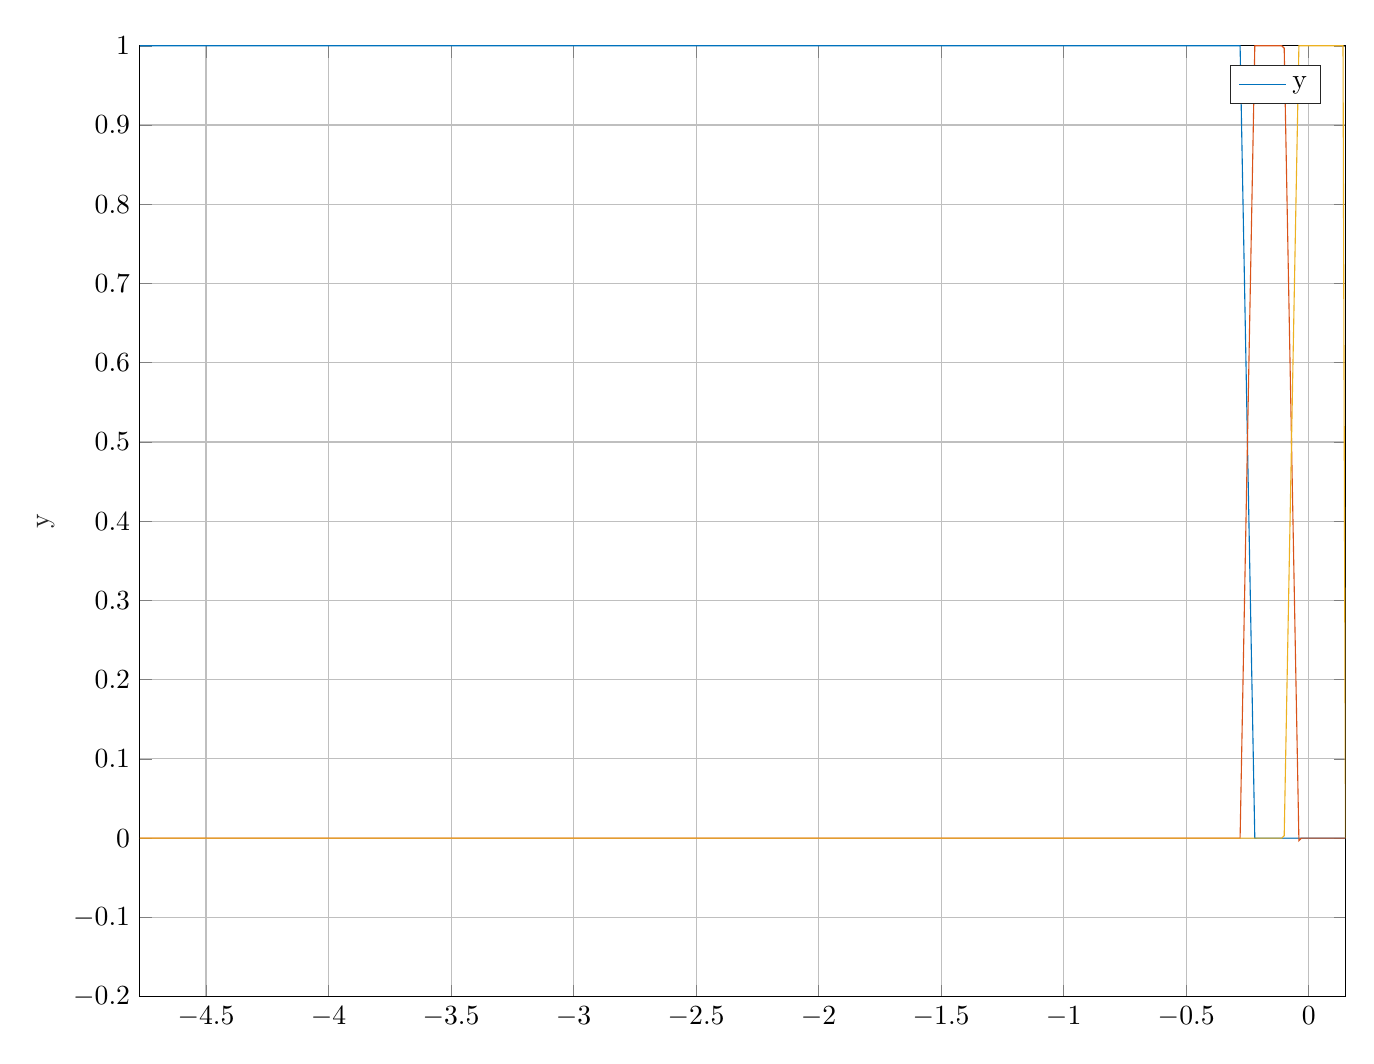
\begin{tikzpicture}

\begin{axis}[%
width=6.028in,
height=4.754in,
at={(1.011in,0.642in)},
scale only axis,
xmin=-4.77,
xmax=0.15,
ymin=-0.2,
ymax=1,
ylabel style={font=\color{white!15!black}},
ylabel={y},
axis background/.style={fill=white},
xmajorgrids,
ymajorgrids,
legend style={legend cell align=left, align=left, draw=white!15!black}
]
\addplot [color=mycolor1]
  table[row sep=crcr]{%
-4.77	1\\
-4.76	1\\
-4.75	1\\
-4.74	1\\
-4.73	1\\
-4.72	1\\
-4.71	1\\
-4.7	1\\
-4.69	1\\
-4.68	1\\
-4.67	1\\
-4.66	1\\
-4.65	1\\
-4.64	1\\
-4.63	1\\
-4.62	1\\
-4.61	1\\
-4.6	1\\
-4.59	1\\
-4.58	1\\
-4.57	1\\
-4.56	1\\
-4.55	1\\
-4.54	1\\
-4.53	1\\
-4.52	1\\
-4.51	1\\
-4.5	1\\
-4.49	1\\
-4.48	1\\
-4.47	1\\
-4.46	1\\
-4.45	1\\
-4.44	1\\
-4.43	1\\
-4.42	1\\
-4.41	1\\
-4.4	1\\
-4.39	1\\
-4.38	1\\
-4.37	1\\
-4.36	1\\
-4.35	1\\
-4.34	1\\
-4.33	1\\
-4.32	1\\
-4.31	1\\
-4.3	1\\
-4.29	1\\
-4.28	1\\
-4.27	1\\
-4.26	1\\
-4.25	1\\
-4.24	1\\
-4.23	1\\
-4.22	1\\
-4.21	1\\
-4.2	1\\
-4.19	1\\
-4.18	1\\
-4.17	1\\
-4.16	1\\
-4.15	1\\
-4.14	1\\
-4.13	1\\
-4.12	1\\
-4.11	1\\
-4.1	1\\
-4.09	1\\
-4.08	1\\
-4.07	1\\
-4.06	1\\
-4.05	1\\
-4.04	1\\
-4.03	1\\
-4.02	1\\
-4.01	1\\
-4	1\\
-3.99	1\\
-3.98	1\\
-3.97	1\\
-3.96	1\\
-3.95	1\\
-3.94	1\\
-3.93	1\\
-3.92	1\\
-3.91	1\\
-3.9	1\\
-3.89	1\\
-3.88	1\\
-3.87	1\\
-3.86	1\\
-3.85	1\\
-3.84	1\\
-3.83	1\\
-3.82	1\\
-3.81	1\\
-3.8	1\\
-3.79	1\\
-3.78	1\\
-3.77	1\\
-3.76	1\\
-3.75	1\\
-3.74	1\\
-3.73	1\\
-3.72	1\\
-3.71	1\\
-3.7	1\\
-3.69	1\\
-3.68	1\\
-3.67	1\\
-3.66	1\\
-3.65	1\\
-3.64	1\\
-3.63	1\\
-3.62	1\\
-3.61	1\\
-3.6	1\\
-3.59	1\\
-3.58	1\\
-3.57	1\\
-3.56	1\\
-3.55	1\\
-3.54	1\\
-3.53	1\\
-3.52	1\\
-3.51	1\\
-3.5	1\\
-3.49	1\\
-3.48	1\\
-3.47	1\\
-3.46	1\\
-3.45	1\\
-3.44	1\\
-3.43	1\\
-3.42	1\\
-3.41	1\\
-3.4	1\\
-3.39	1\\
-3.38	1\\
-3.37	1\\
-3.36	1\\
-3.35	1\\
-3.34	1\\
-3.33	1\\
-3.32	1\\
-3.31	1\\
-3.3	1\\
-3.29	1\\
-3.28	1\\
-3.27	1\\
-3.26	1\\
-3.25	1\\
-3.24	1\\
-3.23	1\\
-3.22	1\\
-3.21	1\\
-3.2	1\\
-3.19	1\\
-3.18	1\\
-3.17	1\\
-3.16	1\\
-3.15	1\\
-3.14	1\\
-3.13	1\\
-3.12	1\\
-3.11	1\\
-3.1	1\\
-3.09	1\\
-3.08	1\\
-3.07	1\\
-3.06	1\\
-3.05	1\\
-3.04	1\\
-3.03	1\\
-3.02	1\\
-3.01	1\\
-3	1\\
-2.99	1\\
-2.98	1\\
-2.97	1\\
-2.96	1\\
-2.95	1\\
-2.94	1\\
-2.93	1\\
-2.92	1\\
-2.91	1\\
-2.9	1\\
-2.89	1\\
-2.88	1\\
-2.87	1\\
-2.86	1\\
-2.85	1\\
-2.84	1\\
-2.83	1\\
-2.82	1\\
-2.81	1\\
-2.8	1\\
-2.79	1\\
-2.78	1\\
-2.77	1\\
-2.76	1\\
-2.75	1\\
-2.74	1\\
-2.73	1\\
-2.72	1\\
-2.71	1\\
-2.7	1\\
-2.69	1\\
-2.68	1\\
-2.67	1\\
-2.66	1\\
-2.65	1\\
-2.64	1\\
-2.63	1\\
-2.62	1\\
-2.61	1\\
-2.6	1\\
-2.59	1\\
-2.58	1\\
-2.57	1\\
-2.56	1\\
-2.55	1\\
-2.54	1\\
-2.53	1\\
-2.52	1\\
-2.51	1\\
-2.5	1\\
-2.49	1\\
-2.48	1\\
-2.47	1\\
-2.46	1\\
-2.45	1\\
-2.44	1\\
-2.43	1\\
-2.42	1\\
-2.41	1\\
-2.4	1\\
-2.39	1\\
-2.38	1\\
-2.37	1\\
-2.36	1\\
-2.35	1\\
-2.34	1\\
-2.33	1\\
-2.32	1\\
-2.31	1\\
-2.3	1\\
-2.29	1\\
-2.28	1\\
-2.27	1\\
-2.26	1\\
-2.25	1\\
-2.24	1\\
-2.23	1\\
-2.22	1\\
-2.21	1\\
-2.2	1\\
-2.19	1\\
-2.18	1\\
-2.17	1\\
-2.16	1\\
-2.15	1\\
-2.14	1\\
-2.13	1\\
-2.12	1\\
-2.11	1\\
-2.1	1\\
-2.09	1\\
-2.08	1\\
-2.07	1\\
-2.06	1\\
-2.05	1\\
-2.04	1\\
-2.03	1\\
-2.02	1\\
-2.01	1\\
-2	1\\
-1.99	1\\
-1.98	1\\
-1.97	1\\
-1.96	1\\
-1.95	1\\
-1.94	1\\
-1.93	1\\
-1.92	1\\
-1.91	1\\
-1.9	1\\
-1.89	1\\
-1.88	1\\
-1.87	1\\
-1.86	1\\
-1.85	1\\
-1.84	1\\
-1.83	1\\
-1.82	1\\
-1.81	1\\
-1.8	1\\
-1.79	1\\
-1.78	1\\
-1.77	1\\
-1.76	1\\
-1.75	1\\
-1.74	1\\
-1.73	1\\
-1.72	1\\
-1.71	1\\
-1.7	1\\
-1.69	1\\
-1.68	1\\
-1.67	1\\
-1.66	1\\
-1.65	1\\
-1.64	1\\
-1.63	1\\
-1.62	1\\
-1.61	1\\
-1.6	1\\
-1.59	1\\
-1.58	1\\
-1.57	1\\
-1.56	1\\
-1.55	1\\
-1.54	1\\
-1.53	1\\
-1.52	1\\
-1.51	1\\
-1.5	1\\
-1.49	1\\
-1.48	1\\
-1.47	1\\
-1.46	1\\
-1.45	1\\
-1.44	1\\
-1.43	1\\
-1.42	1\\
-1.41	1\\
-1.4	1\\
-1.39	1\\
-1.38	1\\
-1.37	1\\
-1.36	1\\
-1.35	1\\
-1.34	1\\
-1.33	1\\
-1.32	1\\
-1.31	1\\
-1.3	1\\
-1.29	1\\
-1.28	1\\
-1.27	1\\
-1.26	1\\
-1.25	1\\
-1.24	1\\
-1.23	1\\
-1.22	1\\
-1.21	1\\
-1.2	1\\
-1.19	1\\
-1.18	1\\
-1.17	1\\
-1.16	1\\
-1.15	1\\
-1.14	1\\
-1.13	1\\
-1.12	1\\
-1.11	1\\
-1.1	1\\
-1.09	1\\
-1.08	1\\
-1.07	1\\
-1.06	1\\
-1.05	1\\
-1.04	1\\
-1.03	1\\
-1.02	1\\
-1.01	1\\
-1	1\\
-0.99	1\\
-0.98	1\\
-0.97	1\\
-0.96	1\\
-0.95	1\\
-0.94	1\\
-0.93	1\\
-0.92	1\\
-0.91	1\\
-0.9	1\\
-0.89	1\\
-0.88	1\\
-0.87	1\\
-0.86	1\\
-0.85	1\\
-0.84	1\\
-0.83	1\\
-0.82	1\\
-0.81	1\\
-0.8	1\\
-0.79	1\\
-0.78	1\\
-0.77	1\\
-0.76	1\\
-0.75	1\\
-0.74	1\\
-0.73	1\\
-0.72	1\\
-0.71	1\\
-0.7	1\\
-0.69	1\\
-0.68	1\\
-0.67	1\\
-0.66	1\\
-0.65	1\\
-0.64	1\\
-0.63	1\\
-0.62	1\\
-0.61	1\\
-0.6	1\\
-0.59	1\\
-0.58	1\\
-0.57	1\\
-0.56	1\\
-0.55	1\\
-0.54	1\\
-0.53	1\\
-0.52	1\\
-0.51	1\\
-0.5	1\\
-0.49	1\\
-0.48	1\\
-0.47	1\\
-0.46	1\\
-0.45	1\\
-0.44	1\\
-0.43	1\\
-0.42	1\\
-0.41	1\\
-0.4	1\\
-0.39	1\\
-0.38	1\\
-0.37	1\\
-0.36	1\\
-0.35	1\\
-0.34	1\\
-0.33	1\\
-0.32	1\\
-0.31	1\\
-0.3	1\\
-0.29	1\\
-0.28	1\\
-0.27	0.8333\\
-0.26	0.6666\\
-0.25	0.4999\\
-0.24	0.3332\\
-0.23	0.1665\\
-0.22	-0.0002\\
-0.21	0\\
-0.2	0\\
-0.19	0\\
-0.18	0\\
-0.17	0\\
-0.16	0\\
-0.15	0\\
-0.14	0\\
-0.13	0\\
-0.12	0\\
-0.11	0\\
-0.1	0\\
-0.09	0\\
-0.08	0\\
-0.07	0\\
-0.06	0\\
-0.05	0\\
-0.04	0\\
-0.03	0\\
-0.02	0\\
-0.01	0\\
0	0\\
0.01	0\\
0.02	0\\
0.03	0\\
0.04	0\\
0.05	0\\
0.06	0\\
0.07	0\\
0.08	0\\
0.09	0\\
0.1	0\\
0.11	0\\
0.12	0\\
0.13	0\\
0.14	0\\
0.15	0\\
};
\addlegendentry{y}

\addplot [color=mycolor2, forget plot]
  table[row sep=crcr]{%
-4.77	0\\
-4.76	0\\
-4.75	0\\
-4.74	0\\
-4.73	0\\
-4.72	0\\
-4.71	0\\
-4.7	0\\
-4.69	0\\
-4.68	0\\
-4.67	0\\
-4.66	0\\
-4.65	0\\
-4.64	0\\
-4.63	0\\
-4.62	0\\
-4.61	0\\
-4.6	0\\
-4.59	0\\
-4.58	0\\
-4.57	0\\
-4.56	0\\
-4.55	0\\
-4.54	0\\
-4.53	0\\
-4.52	0\\
-4.51	0\\
-4.5	0\\
-4.49	0\\
-4.48	0\\
-4.47	0\\
-4.46	0\\
-4.45	0\\
-4.44	0\\
-4.43	0\\
-4.42	0\\
-4.41	0\\
-4.4	0\\
-4.39	0\\
-4.38	0\\
-4.37	0\\
-4.36	0\\
-4.35	0\\
-4.34	0\\
-4.33	0\\
-4.32	0\\
-4.31	0\\
-4.3	0\\
-4.29	0\\
-4.28	0\\
-4.27	0\\
-4.26	0\\
-4.25	0\\
-4.24	0\\
-4.23	0\\
-4.22	0\\
-4.21	0\\
-4.2	0\\
-4.19	0\\
-4.18	0\\
-4.17	0\\
-4.16	0\\
-4.15	0\\
-4.14	0\\
-4.13	0\\
-4.12	0\\
-4.11	0\\
-4.1	0\\
-4.09	0\\
-4.08	0\\
-4.07	0\\
-4.06	0\\
-4.05	0\\
-4.04	0\\
-4.03	0\\
-4.02	0\\
-4.01	0\\
-4	0\\
-3.99	0\\
-3.98	0\\
-3.97	0\\
-3.96	0\\
-3.95	0\\
-3.94	0\\
-3.93	0\\
-3.92	0\\
-3.91	0\\
-3.9	0\\
-3.89	0\\
-3.88	0\\
-3.87	0\\
-3.86	0\\
-3.85	0\\
-3.84	0\\
-3.83	0\\
-3.82	0\\
-3.81	0\\
-3.8	0\\
-3.79	0\\
-3.78	0\\
-3.77	0\\
-3.76	0\\
-3.75	0\\
-3.74	0\\
-3.73	0\\
-3.72	0\\
-3.71	0\\
-3.7	0\\
-3.69	0\\
-3.68	0\\
-3.67	0\\
-3.66	0\\
-3.65	0\\
-3.64	0\\
-3.63	0\\
-3.62	0\\
-3.61	0\\
-3.6	0\\
-3.59	0\\
-3.58	0\\
-3.57	0\\
-3.56	0\\
-3.55	0\\
-3.54	0\\
-3.53	0\\
-3.52	0\\
-3.51	0\\
-3.5	0\\
-3.49	0\\
-3.48	0\\
-3.47	0\\
-3.46	0\\
-3.45	0\\
-3.44	0\\
-3.43	0\\
-3.42	0\\
-3.41	0\\
-3.4	0\\
-3.39	0\\
-3.38	0\\
-3.37	0\\
-3.36	0\\
-3.35	0\\
-3.34	0\\
-3.33	0\\
-3.32	0\\
-3.31	0\\
-3.3	0\\
-3.29	0\\
-3.28	0\\
-3.27	0\\
-3.26	0\\
-3.25	0\\
-3.24	0\\
-3.23	0\\
-3.22	0\\
-3.21	0\\
-3.2	0\\
-3.19	0\\
-3.18	0\\
-3.17	0\\
-3.16	0\\
-3.15	0\\
-3.14	0\\
-3.13	0\\
-3.12	0\\
-3.11	0\\
-3.1	0\\
-3.09	0\\
-3.08	0\\
-3.07	0\\
-3.06	0\\
-3.05	0\\
-3.04	0\\
-3.03	0\\
-3.02	0\\
-3.01	0\\
-3	0\\
-2.99	0\\
-2.98	0\\
-2.97	0\\
-2.96	0\\
-2.95	0\\
-2.94	0\\
-2.93	0\\
-2.92	0\\
-2.91	0\\
-2.9	0\\
-2.89	0\\
-2.88	0\\
-2.87	0\\
-2.86	0\\
-2.85	0\\
-2.84	0\\
-2.83	0\\
-2.82	0\\
-2.81	0\\
-2.8	0\\
-2.79	0\\
-2.78	0\\
-2.77	0\\
-2.76	0\\
-2.75	0\\
-2.74	0\\
-2.73	0\\
-2.72	0\\
-2.71	0\\
-2.7	0\\
-2.69	0\\
-2.68	0\\
-2.67	0\\
-2.66	0\\
-2.65	0\\
-2.64	0\\
-2.63	0\\
-2.62	0\\
-2.61	0\\
-2.6	0\\
-2.59	0\\
-2.58	0\\
-2.57	0\\
-2.56	0\\
-2.55	0\\
-2.54	0\\
-2.53	0\\
-2.52	0\\
-2.51	0\\
-2.5	0\\
-2.49	0\\
-2.48	0\\
-2.47	0\\
-2.46	0\\
-2.45	0\\
-2.44	0\\
-2.43	0\\
-2.42	0\\
-2.41	0\\
-2.4	0\\
-2.39	0\\
-2.38	0\\
-2.37	0\\
-2.36	0\\
-2.35	0\\
-2.34	0\\
-2.33	0\\
-2.32	0\\
-2.31	0\\
-2.3	0\\
-2.29	0\\
-2.28	0\\
-2.27	0\\
-2.26	0\\
-2.25	0\\
-2.24	0\\
-2.23	0\\
-2.22	0\\
-2.21	0\\
-2.2	0\\
-2.19	0\\
-2.18	0\\
-2.17	0\\
-2.16	0\\
-2.15	0\\
-2.14	0\\
-2.13	0\\
-2.12	0\\
-2.11	0\\
-2.1	0\\
-2.09	0\\
-2.08	0\\
-2.07	0\\
-2.06	0\\
-2.05	0\\
-2.04	0\\
-2.03	0\\
-2.02	0\\
-2.01	0\\
-2	0\\
-1.99	0\\
-1.98	0\\
-1.97	0\\
-1.96	0\\
-1.95	0\\
-1.94	0\\
-1.93	0\\
-1.92	0\\
-1.91	0\\
-1.9	0\\
-1.89	0\\
-1.88	0\\
-1.87	0\\
-1.86	0\\
-1.85	0\\
-1.84	0\\
-1.83	0\\
-1.82	0\\
-1.81	0\\
-1.8	0\\
-1.79	0\\
-1.78	0\\
-1.77	0\\
-1.76	0\\
-1.75	0\\
-1.74	0\\
-1.73	0\\
-1.72	0\\
-1.71	0\\
-1.7	0\\
-1.69	0\\
-1.68	0\\
-1.67	0\\
-1.66	0\\
-1.65	0\\
-1.64	0\\
-1.63	0\\
-1.62	0\\
-1.61	0\\
-1.6	0\\
-1.59	0\\
-1.58	0\\
-1.57	0\\
-1.56	0\\
-1.55	0\\
-1.54	0\\
-1.53	0\\
-1.52	0\\
-1.51	0\\
-1.5	0\\
-1.49	0\\
-1.48	0\\
-1.47	0\\
-1.46	0\\
-1.45	0\\
-1.44	0\\
-1.43	0\\
-1.42	0\\
-1.41	0\\
-1.4	0\\
-1.39	0\\
-1.38	0\\
-1.37	0\\
-1.36	0\\
-1.35	0\\
-1.34	0\\
-1.33	0\\
-1.32	0\\
-1.31	0\\
-1.3	0\\
-1.29	0\\
-1.28	0\\
-1.27	0\\
-1.26	0\\
-1.25	0\\
-1.24	0\\
-1.23	0\\
-1.22	0\\
-1.21	0\\
-1.2	0\\
-1.19	0\\
-1.18	0\\
-1.17	0\\
-1.16	0\\
-1.15	0\\
-1.14	0\\
-1.13	0\\
-1.12	0\\
-1.11	0\\
-1.1	0\\
-1.09	0\\
-1.08	0\\
-1.07	0\\
-1.06	0\\
-1.05	0\\
-1.04	0\\
-1.03	0\\
-1.02	0\\
-1.01	0\\
-1	0\\
-0.99	0\\
-0.98	0\\
-0.97	0\\
-0.96	0\\
-0.95	0\\
-0.94	0\\
-0.93	0\\
-0.92	0\\
-0.91	0\\
-0.9	0\\
-0.89	0\\
-0.88	0\\
-0.87	0\\
-0.86	0\\
-0.85	0\\
-0.84	0\\
-0.83	0\\
-0.82	0\\
-0.81	0\\
-0.8	0\\
-0.79	0\\
-0.78	0\\
-0.77	0\\
-0.76	0\\
-0.75	0\\
-0.74	0\\
-0.73	0\\
-0.72	0\\
-0.71	0\\
-0.7	0\\
-0.69	0\\
-0.68	0\\
-0.67	0\\
-0.66	0\\
-0.65	0\\
-0.64	0\\
-0.63	0\\
-0.62	0\\
-0.61	0\\
-0.6	0\\
-0.59	0\\
-0.58	0\\
-0.57	0\\
-0.56	0\\
-0.55	0\\
-0.54	0\\
-0.53	0\\
-0.52	0\\
-0.51	0\\
-0.5	0\\
-0.49	0\\
-0.48	0\\
-0.47	0\\
-0.46	0\\
-0.45	0\\
-0.44	0\\
-0.43	0\\
-0.42	0\\
-0.41	0\\
-0.4	0\\
-0.39	0\\
-0.38	0\\
-0.37	0\\
-0.36	0\\
-0.35	0\\
-0.34	0\\
-0.33	0\\
-0.32	0\\
-0.31	0\\
-0.3	0\\
-0.29	0\\
-0.28	0\\
-0.27	0.1667\\
-0.26	0.3334\\
-0.25	0.5001\\
-0.24	0.6668\\
-0.23	0.8335\\
-0.22	1\\
-0.21	1\\
-0.2	1\\
-0.19	1\\
-0.18	1\\
-0.17	1\\
-0.16	1\\
-0.15	1\\
-0.14	1\\
-0.13	1\\
-0.12	1\\
-0.11	1\\
-0.1	0.997\\
-0.09	0.8303\\
-0.08	0.6636\\
-0.07	0.4969\\
-0.06	0.3302\\
-0.05	0.1635\\
-0.04	-0.0032\\
-0.03	0\\
-0.02	0\\
-0.01	0\\
0	0\\
0.01	0\\
0.02	0\\
0.03	0\\
0.04	0\\
0.05	0\\
0.06	0\\
0.07	0\\
0.08	0\\
0.09	0\\
0.1	0\\
0.11	0\\
0.12	0\\
0.13	0\\
0.14	0\\
0.15	0\\
};
\addplot [color=mycolor3, forget plot]
  table[row sep=crcr]{%
-4.77	0\\
-4.76	0\\
-4.75	0\\
-4.74	0\\
-4.73	0\\
-4.72	0\\
-4.71	0\\
-4.7	0\\
-4.69	0\\
-4.68	0\\
-4.67	0\\
-4.66	0\\
-4.65	0\\
-4.64	0\\
-4.63	0\\
-4.62	0\\
-4.61	0\\
-4.6	0\\
-4.59	0\\
-4.58	0\\
-4.57	0\\
-4.56	0\\
-4.55	0\\
-4.54	0\\
-4.53	0\\
-4.52	0\\
-4.51	0\\
-4.5	0\\
-4.49	0\\
-4.48	0\\
-4.47	0\\
-4.46	0\\
-4.45	0\\
-4.44	0\\
-4.43	0\\
-4.42	0\\
-4.41	0\\
-4.4	0\\
-4.39	0\\
-4.38	0\\
-4.37	0\\
-4.36	0\\
-4.35	0\\
-4.34	0\\
-4.33	0\\
-4.32	0\\
-4.31	0\\
-4.3	0\\
-4.29	0\\
-4.28	0\\
-4.27	0\\
-4.26	0\\
-4.25	0\\
-4.24	0\\
-4.23	0\\
-4.22	0\\
-4.21	0\\
-4.2	0\\
-4.19	0\\
-4.18	0\\
-4.17	0\\
-4.16	0\\
-4.15	0\\
-4.14	0\\
-4.13	0\\
-4.12	0\\
-4.11	0\\
-4.1	0\\
-4.09	0\\
-4.08	0\\
-4.07	0\\
-4.06	0\\
-4.05	0\\
-4.04	0\\
-4.03	0\\
-4.02	0\\
-4.01	0\\
-4	0\\
-3.99	0\\
-3.98	0\\
-3.97	0\\
-3.96	0\\
-3.95	0\\
-3.94	0\\
-3.93	0\\
-3.92	0\\
-3.91	0\\
-3.9	0\\
-3.89	0\\
-3.88	0\\
-3.87	0\\
-3.86	0\\
-3.85	0\\
-3.84	0\\
-3.83	0\\
-3.82	0\\
-3.81	0\\
-3.8	0\\
-3.79	0\\
-3.78	0\\
-3.77	0\\
-3.76	0\\
-3.75	0\\
-3.74	0\\
-3.73	0\\
-3.72	0\\
-3.71	0\\
-3.7	0\\
-3.69	0\\
-3.68	0\\
-3.67	0\\
-3.66	0\\
-3.65	0\\
-3.64	0\\
-3.63	0\\
-3.62	0\\
-3.61	0\\
-3.6	0\\
-3.59	0\\
-3.58	0\\
-3.57	0\\
-3.56	0\\
-3.55	0\\
-3.54	0\\
-3.53	0\\
-3.52	0\\
-3.51	0\\
-3.5	0\\
-3.49	0\\
-3.48	0\\
-3.47	0\\
-3.46	0\\
-3.45	0\\
-3.44	0\\
-3.43	0\\
-3.42	0\\
-3.41	0\\
-3.4	0\\
-3.39	0\\
-3.38	0\\
-3.37	0\\
-3.36	0\\
-3.35	0\\
-3.34	0\\
-3.33	0\\
-3.32	0\\
-3.31	0\\
-3.3	0\\
-3.29	0\\
-3.28	0\\
-3.27	0\\
-3.26	0\\
-3.25	0\\
-3.24	0\\
-3.23	0\\
-3.22	0\\
-3.21	0\\
-3.2	0\\
-3.19	0\\
-3.18	0\\
-3.17	0\\
-3.16	0\\
-3.15	0\\
-3.14	0\\
-3.13	0\\
-3.12	0\\
-3.11	0\\
-3.1	0\\
-3.09	0\\
-3.08	0\\
-3.07	0\\
-3.06	0\\
-3.05	0\\
-3.04	0\\
-3.03	0\\
-3.02	0\\
-3.01	0\\
-3	0\\
-2.99	0\\
-2.98	0\\
-2.97	0\\
-2.96	0\\
-2.95	0\\
-2.94	0\\
-2.93	0\\
-2.92	0\\
-2.91	0\\
-2.9	0\\
-2.89	0\\
-2.88	0\\
-2.87	0\\
-2.86	0\\
-2.85	0\\
-2.84	0\\
-2.83	0\\
-2.82	0\\
-2.81	0\\
-2.8	0\\
-2.79	0\\
-2.78	0\\
-2.77	0\\
-2.76	0\\
-2.75	0\\
-2.74	0\\
-2.73	0\\
-2.72	0\\
-2.71	0\\
-2.7	0\\
-2.69	0\\
-2.68	0\\
-2.67	0\\
-2.66	0\\
-2.65	0\\
-2.64	0\\
-2.63	0\\
-2.62	0\\
-2.61	0\\
-2.6	0\\
-2.59	0\\
-2.58	0\\
-2.57	0\\
-2.56	0\\
-2.55	0\\
-2.54	0\\
-2.53	0\\
-2.52	0\\
-2.51	0\\
-2.5	0\\
-2.49	0\\
-2.48	0\\
-2.47	0\\
-2.46	0\\
-2.45	0\\
-2.44	0\\
-2.43	0\\
-2.42	0\\
-2.41	0\\
-2.4	0\\
-2.39	0\\
-2.38	0\\
-2.37	0\\
-2.36	0\\
-2.35	0\\
-2.34	0\\
-2.33	0\\
-2.32	0\\
-2.31	0\\
-2.3	0\\
-2.29	0\\
-2.28	0\\
-2.27	0\\
-2.26	0\\
-2.25	0\\
-2.24	0\\
-2.23	0\\
-2.22	0\\
-2.21	0\\
-2.2	0\\
-2.19	0\\
-2.18	0\\
-2.17	0\\
-2.16	0\\
-2.15	0\\
-2.14	0\\
-2.13	0\\
-2.12	0\\
-2.11	0\\
-2.1	0\\
-2.09	0\\
-2.08	0\\
-2.07	0\\
-2.06	0\\
-2.05	0\\
-2.04	0\\
-2.03	0\\
-2.02	0\\
-2.01	0\\
-2	0\\
-1.99	0\\
-1.98	0\\
-1.97	0\\
-1.96	0\\
-1.95	0\\
-1.94	0\\
-1.93	0\\
-1.92	0\\
-1.91	0\\
-1.9	0\\
-1.89	0\\
-1.88	0\\
-1.87	0\\
-1.86	0\\
-1.85	0\\
-1.84	0\\
-1.83	0\\
-1.82	0\\
-1.81	0\\
-1.8	0\\
-1.79	0\\
-1.78	0\\
-1.77	0\\
-1.76	0\\
-1.75	0\\
-1.74	0\\
-1.73	0\\
-1.72	0\\
-1.71	0\\
-1.7	0\\
-1.69	0\\
-1.68	0\\
-1.67	0\\
-1.66	0\\
-1.65	0\\
-1.64	0\\
-1.63	0\\
-1.62	0\\
-1.61	0\\
-1.6	0\\
-1.59	0\\
-1.58	0\\
-1.57	0\\
-1.56	0\\
-1.55	0\\
-1.54	0\\
-1.53	0\\
-1.52	0\\
-1.51	0\\
-1.5	0\\
-1.49	0\\
-1.48	0\\
-1.47	0\\
-1.46	0\\
-1.45	0\\
-1.44	0\\
-1.43	0\\
-1.42	0\\
-1.41	0\\
-1.4	0\\
-1.39	0\\
-1.38	0\\
-1.37	0\\
-1.36	0\\
-1.35	0\\
-1.34	0\\
-1.33	0\\
-1.32	0\\
-1.31	0\\
-1.3	0\\
-1.29	0\\
-1.28	0\\
-1.27	0\\
-1.26	0\\
-1.25	0\\
-1.24	0\\
-1.23	0\\
-1.22	0\\
-1.21	0\\
-1.2	0\\
-1.19	0\\
-1.18	0\\
-1.17	0\\
-1.16	0\\
-1.15	0\\
-1.14	0\\
-1.13	0\\
-1.12	0\\
-1.11	0\\
-1.1	0\\
-1.09	0\\
-1.08	0\\
-1.07	0\\
-1.06	0\\
-1.05	0\\
-1.04	0\\
-1.03	0\\
-1.02	0\\
-1.01	0\\
-1	0\\
-0.99	0\\
-0.98	0\\
-0.97	0\\
-0.96	0\\
-0.95	0\\
-0.94	0\\
-0.93	0\\
-0.92	0\\
-0.91	0\\
-0.9	0\\
-0.89	0\\
-0.88	0\\
-0.87	0\\
-0.86	0\\
-0.85	0\\
-0.84	0\\
-0.83	0\\
-0.82	0\\
-0.81	0\\
-0.8	0\\
-0.79	0\\
-0.78	0\\
-0.77	0\\
-0.76	0\\
-0.75	0\\
-0.74	0\\
-0.73	0\\
-0.72	0\\
-0.71	0\\
-0.7	0\\
-0.69	0\\
-0.68	0\\
-0.67	0\\
-0.66	0\\
-0.65	0\\
-0.64	0\\
-0.63	0\\
-0.62	0\\
-0.61	0\\
-0.6	0\\
-0.59	0\\
-0.58	0\\
-0.57	0\\
-0.56	0\\
-0.55	0\\
-0.54	0\\
-0.53	0\\
-0.52	0\\
-0.51	0\\
-0.5	0\\
-0.49	0\\
-0.48	0\\
-0.47	0\\
-0.46	0\\
-0.45	0\\
-0.44	0\\
-0.43	0\\
-0.42	0\\
-0.41	0\\
-0.4	0\\
-0.39	0\\
-0.38	0\\
-0.37	0\\
-0.36	0\\
-0.35	0\\
-0.34	0\\
-0.33	0\\
-0.32	0\\
-0.31	0\\
-0.3	0\\
-0.29	0\\
-0.28	0\\
-0.27	0\\
-0.26	0\\
-0.25	0\\
-0.24	0\\
-0.23	0\\
-0.22	0\\
-0.21	0\\
-0.2	0\\
-0.19	0\\
-0.18	0\\
-0.17	0\\
-0.16	0\\
-0.15	0\\
-0.14	0\\
-0.13	0\\
-0.12	0\\
-0.11	0\\
-0.1	0.003\\
-0.09	0.1697\\
-0.08	0.3364\\
-0.07	0.5031\\
-0.06	0.6698\\
-0.05	0.8365\\
-0.04	1\\
-0.03	1\\
-0.02	1\\
-0.01	1\\
0	1\\
0.01	1\\
0.02	1\\
0.03	1\\
0.04	1\\
0.05	1\\
0.06	1\\
0.07	1\\
0.08	1\\
0.09	1\\
0.1	1\\
0.11	1\\
0.12	1\\
0.13	1\\
0.14	1\\
0.15	0\\
};
\end{axis}
\end{tikzpicture}%
    \caption{Funkcje rozmycia dla 3 regulatorów lokalnych}
    \label{lab:zad4:fuzzyFunction:3:figure}
\end{figure}

\begin{figure}[H] 
    \centering
    % This file was created by matlab2tikz.
%
\definecolor{mycolor1}{rgb}{0.00000,0.44700,0.74100}%
\definecolor{mycolor2}{rgb}{0.85000,0.32500,0.09800}%
\definecolor{mycolor3}{rgb}{0.92900,0.69400,0.12500}%
\definecolor{mycolor4}{rgb}{0.49400,0.18400,0.55600}%
%
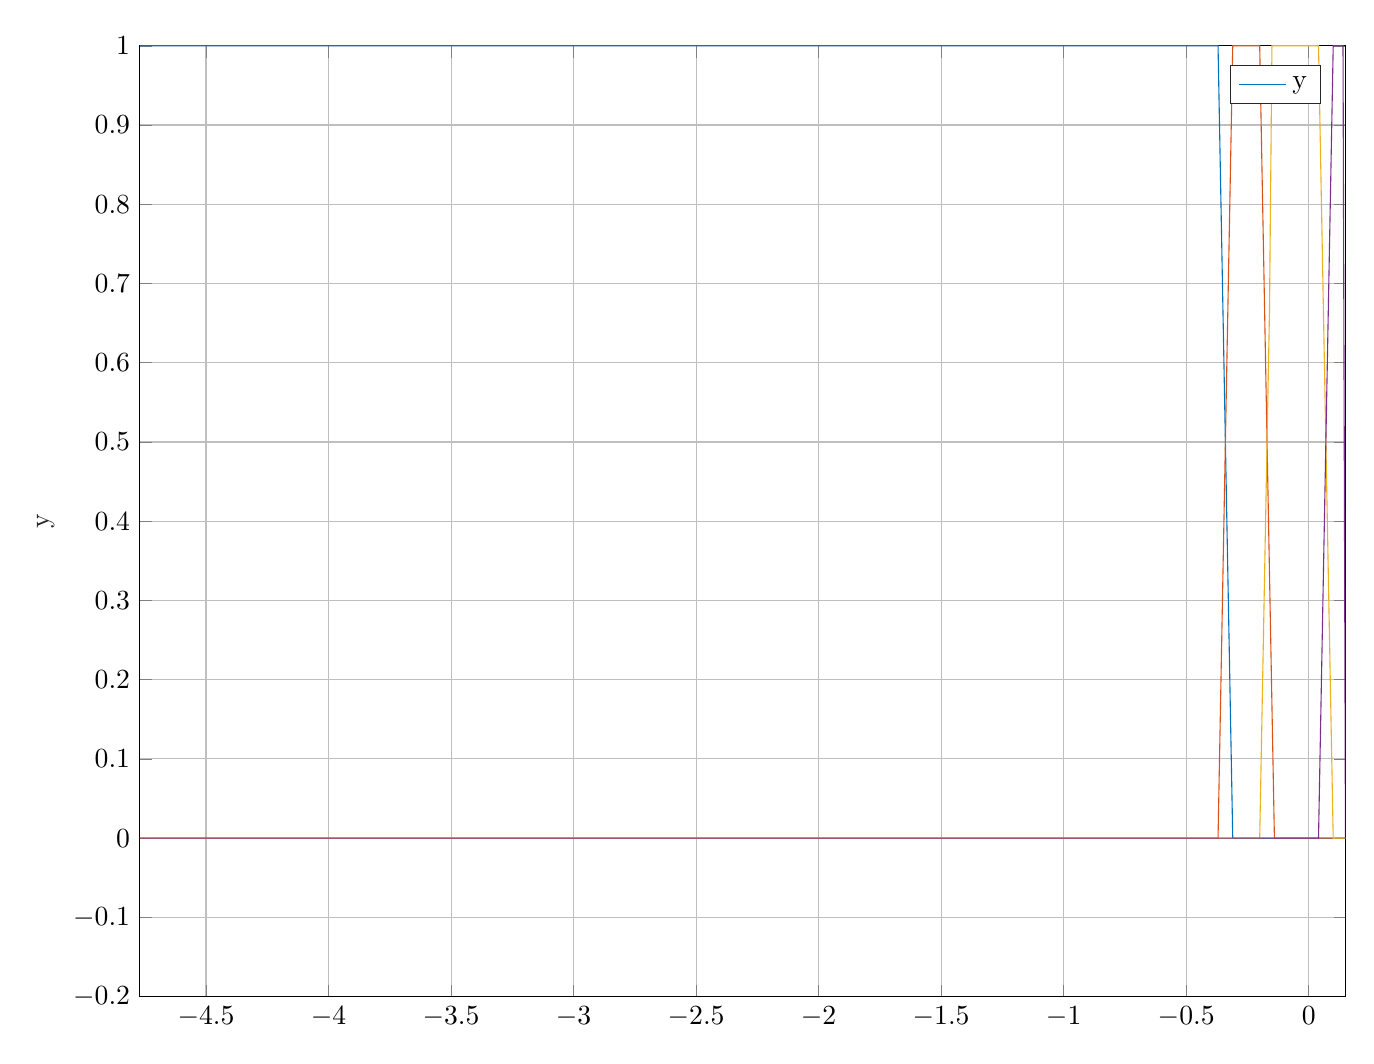
\begin{tikzpicture}

\begin{axis}[%
width=6.028in,
height=4.754in,
at={(1.011in,0.642in)},
scale only axis,
xmin=-4.77,
xmax=0.15,
ymin=-0.2,
ymax=1,
ylabel style={font=\color{white!15!black}},
ylabel={y},
axis background/.style={fill=white},
xmajorgrids,
ymajorgrids,
legend style={legend cell align=left, align=left, draw=white!15!black}
]
\addplot [color=mycolor1]
  table[row sep=crcr]{%
-4.77	1\\
-4.76	1\\
-4.75	1\\
-4.74	1\\
-4.73	1\\
-4.72	1\\
-4.71	1\\
-4.7	1\\
-4.69	1\\
-4.68	1\\
-4.67	1\\
-4.66	1\\
-4.65	1\\
-4.64	1\\
-4.63	1\\
-4.62	1\\
-4.61	1\\
-4.6	1\\
-4.59	1\\
-4.58	1\\
-4.57	1\\
-4.56	1\\
-4.55	1\\
-4.54	1\\
-4.53	1\\
-4.52	1\\
-4.51	1\\
-4.5	1\\
-4.49	1\\
-4.48	1\\
-4.47	1\\
-4.46	1\\
-4.45	1\\
-4.44	1\\
-4.43	1\\
-4.42	1\\
-4.41	1\\
-4.4	1\\
-4.39	1\\
-4.38	1\\
-4.37	1\\
-4.36	1\\
-4.35	1\\
-4.34	1\\
-4.33	1\\
-4.32	1\\
-4.31	1\\
-4.3	1\\
-4.29	1\\
-4.28	1\\
-4.27	1\\
-4.26	1\\
-4.25	1\\
-4.24	1\\
-4.23	1\\
-4.22	1\\
-4.21	1\\
-4.2	1\\
-4.19	1\\
-4.18	1\\
-4.17	1\\
-4.16	1\\
-4.15	1\\
-4.14	1\\
-4.13	1\\
-4.12	1\\
-4.11	1\\
-4.1	1\\
-4.09	1\\
-4.08	1\\
-4.07	1\\
-4.06	1\\
-4.05	1\\
-4.04	1\\
-4.03	1\\
-4.02	1\\
-4.01	1\\
-4	1\\
-3.99	1\\
-3.98	1\\
-3.97	1\\
-3.96	1\\
-3.95	1\\
-3.94	1\\
-3.93	1\\
-3.92	1\\
-3.91	1\\
-3.9	1\\
-3.89	1\\
-3.88	1\\
-3.87	1\\
-3.86	1\\
-3.85	1\\
-3.84	1\\
-3.83	1\\
-3.82	1\\
-3.81	1\\
-3.8	1\\
-3.79	1\\
-3.78	1\\
-3.77	1\\
-3.76	1\\
-3.75	1\\
-3.74	1\\
-3.73	1\\
-3.72	1\\
-3.71	1\\
-3.7	1\\
-3.69	1\\
-3.68	1\\
-3.67	1\\
-3.66	1\\
-3.65	1\\
-3.64	1\\
-3.63	1\\
-3.62	1\\
-3.61	1\\
-3.6	1\\
-3.59	1\\
-3.58	1\\
-3.57	1\\
-3.56	1\\
-3.55	1\\
-3.54	1\\
-3.53	1\\
-3.52	1\\
-3.51	1\\
-3.5	1\\
-3.49	1\\
-3.48	1\\
-3.47	1\\
-3.46	1\\
-3.45	1\\
-3.44	1\\
-3.43	1\\
-3.42	1\\
-3.41	1\\
-3.4	1\\
-3.39	1\\
-3.38	1\\
-3.37	1\\
-3.36	1\\
-3.35	1\\
-3.34	1\\
-3.33	1\\
-3.32	1\\
-3.31	1\\
-3.3	1\\
-3.29	1\\
-3.28	1\\
-3.27	1\\
-3.26	1\\
-3.25	1\\
-3.24	1\\
-3.23	1\\
-3.22	1\\
-3.21	1\\
-3.2	1\\
-3.19	1\\
-3.18	1\\
-3.17	1\\
-3.16	1\\
-3.15	1\\
-3.14	1\\
-3.13	1\\
-3.12	1\\
-3.11	1\\
-3.1	1\\
-3.09	1\\
-3.08	1\\
-3.07	1\\
-3.06	1\\
-3.05	1\\
-3.04	1\\
-3.03	1\\
-3.02	1\\
-3.01	1\\
-3	1\\
-2.99	1\\
-2.98	1\\
-2.97	1\\
-2.96	1\\
-2.95	1\\
-2.94	1\\
-2.93	1\\
-2.92	1\\
-2.91	1\\
-2.9	1\\
-2.89	1\\
-2.88	1\\
-2.87	1\\
-2.86	1\\
-2.85	1\\
-2.84	1\\
-2.83	1\\
-2.82	1\\
-2.81	1\\
-2.8	1\\
-2.79	1\\
-2.78	1\\
-2.77	1\\
-2.76	1\\
-2.75	1\\
-2.74	1\\
-2.73	1\\
-2.72	1\\
-2.71	1\\
-2.7	1\\
-2.69	1\\
-2.68	1\\
-2.67	1\\
-2.66	1\\
-2.65	1\\
-2.64	1\\
-2.63	1\\
-2.62	1\\
-2.61	1\\
-2.6	1\\
-2.59	1\\
-2.58	1\\
-2.57	1\\
-2.56	1\\
-2.55	1\\
-2.54	1\\
-2.53	1\\
-2.52	1\\
-2.51	1\\
-2.5	1\\
-2.49	1\\
-2.48	1\\
-2.47	1\\
-2.46	1\\
-2.45	1\\
-2.44	1\\
-2.43	1\\
-2.42	1\\
-2.41	1\\
-2.4	1\\
-2.39	1\\
-2.38	1\\
-2.37	1\\
-2.36	1\\
-2.35	1\\
-2.34	1\\
-2.33	1\\
-2.32	1\\
-2.31	1\\
-2.3	1\\
-2.29	1\\
-2.28	1\\
-2.27	1\\
-2.26	1\\
-2.25	1\\
-2.24	1\\
-2.23	1\\
-2.22	1\\
-2.21	1\\
-2.2	1\\
-2.19	1\\
-2.18	1\\
-2.17	1\\
-2.16	1\\
-2.15	1\\
-2.14	1\\
-2.13	1\\
-2.12	1\\
-2.11	1\\
-2.1	1\\
-2.09	1\\
-2.08	1\\
-2.07	1\\
-2.06	1\\
-2.05	1\\
-2.04	1\\
-2.03	1\\
-2.02	1\\
-2.01	1\\
-2	1\\
-1.99	1\\
-1.98	1\\
-1.97	1\\
-1.96	1\\
-1.95	1\\
-1.94	1\\
-1.93	1\\
-1.92	1\\
-1.91	1\\
-1.9	1\\
-1.89	1\\
-1.88	1\\
-1.87	1\\
-1.86	1\\
-1.85	1\\
-1.84	1\\
-1.83	1\\
-1.82	1\\
-1.81	1\\
-1.8	1\\
-1.79	1\\
-1.78	1\\
-1.77	1\\
-1.76	1\\
-1.75	1\\
-1.74	1\\
-1.73	1\\
-1.72	1\\
-1.71	1\\
-1.7	1\\
-1.69	1\\
-1.68	1\\
-1.67	1\\
-1.66	1\\
-1.65	1\\
-1.64	1\\
-1.63	1\\
-1.62	1\\
-1.61	1\\
-1.6	1\\
-1.59	1\\
-1.58	1\\
-1.57	1\\
-1.56	1\\
-1.55	1\\
-1.54	1\\
-1.53	1\\
-1.52	1\\
-1.51	1\\
-1.5	1\\
-1.49	1\\
-1.48	1\\
-1.47	1\\
-1.46	1\\
-1.45	1\\
-1.44	1\\
-1.43	1\\
-1.42	1\\
-1.41	1\\
-1.4	1\\
-1.39	1\\
-1.38	1\\
-1.37	1\\
-1.36	1\\
-1.35	1\\
-1.34	1\\
-1.33	1\\
-1.32	1\\
-1.31	1\\
-1.3	1\\
-1.29	1\\
-1.28	1\\
-1.27	1\\
-1.26	1\\
-1.25	1\\
-1.24	1\\
-1.23	1\\
-1.22	1\\
-1.21	1\\
-1.2	1\\
-1.19	1\\
-1.18	1\\
-1.17	1\\
-1.16	1\\
-1.15	1\\
-1.14	1\\
-1.13	1\\
-1.12	1\\
-1.11	1\\
-1.1	1\\
-1.09	1\\
-1.08	1\\
-1.07	1\\
-1.06	1\\
-1.05	1\\
-1.04	1\\
-1.03	1\\
-1.02	1\\
-1.01	1\\
-1	1\\
-0.99	1\\
-0.98	1\\
-0.97	1\\
-0.96	1\\
-0.95	1\\
-0.94	1\\
-0.93	1\\
-0.92	1\\
-0.91	1\\
-0.9	1\\
-0.89	1\\
-0.88	1\\
-0.87	1\\
-0.86	1\\
-0.85	1\\
-0.84	1\\
-0.83	1\\
-0.82	1\\
-0.81	1\\
-0.8	1\\
-0.79	1\\
-0.78	1\\
-0.77	1\\
-0.76	1\\
-0.75	1\\
-0.74	1\\
-0.73	1\\
-0.72	1\\
-0.71	1\\
-0.7	1\\
-0.69	1\\
-0.68	1\\
-0.67	1\\
-0.66	1\\
-0.65	1\\
-0.64	1\\
-0.63	1\\
-0.62	1\\
-0.61	1\\
-0.6	1\\
-0.59	1\\
-0.58	1\\
-0.57	1\\
-0.56	1\\
-0.55	1\\
-0.54	1\\
-0.53	1\\
-0.52	1\\
-0.51	1\\
-0.5	1\\
-0.49	1\\
-0.48	1\\
-0.47	1\\
-0.46	1\\
-0.45	1\\
-0.44	1\\
-0.43	1\\
-0.42	1\\
-0.41	1\\
-0.4	1\\
-0.39	1\\
-0.38	1\\
-0.37	1\\
-0.36	0.8333\\
-0.35	0.6666\\
-0.34	0.4999\\
-0.33	0.3332\\
-0.32	0.1665\\
-0.31	-0.0002\\
-0.3	0\\
-0.29	0\\
-0.28	0\\
-0.27	0\\
-0.26	0\\
-0.25	0\\
-0.24	0\\
-0.23	0\\
-0.22	0\\
-0.21	0\\
-0.2	0\\
-0.19	0\\
-0.18	0\\
-0.17	0\\
-0.16	0\\
-0.15	0\\
-0.14	0\\
-0.13	0\\
-0.12	0\\
-0.11	0\\
-0.1	0\\
-0.09	0\\
-0.08	0\\
-0.07	0\\
-0.06	0\\
-0.05	0\\
-0.04	0\\
-0.03	0\\
-0.02	0\\
-0.01	0\\
0	0\\
0.01	0\\
0.02	0\\
0.03	0\\
0.04	0\\
0.05	0\\
0.06	0\\
0.07	0\\
0.08	0\\
0.09	0\\
0.1	0\\
0.11	0\\
0.12	0\\
0.13	0\\
0.14	0\\
0.15	0\\
};
\addlegendentry{y}

\addplot [color=mycolor2, forget plot]
  table[row sep=crcr]{%
-4.77	0\\
-4.76	0\\
-4.75	0\\
-4.74	0\\
-4.73	0\\
-4.72	0\\
-4.71	0\\
-4.7	0\\
-4.69	0\\
-4.68	0\\
-4.67	0\\
-4.66	0\\
-4.65	0\\
-4.64	0\\
-4.63	0\\
-4.62	0\\
-4.61	0\\
-4.6	0\\
-4.59	0\\
-4.58	0\\
-4.57	0\\
-4.56	0\\
-4.55	0\\
-4.54	0\\
-4.53	0\\
-4.52	0\\
-4.51	0\\
-4.5	0\\
-4.49	0\\
-4.48	0\\
-4.47	0\\
-4.46	0\\
-4.45	0\\
-4.44	0\\
-4.43	0\\
-4.42	0\\
-4.41	0\\
-4.4	0\\
-4.39	0\\
-4.38	0\\
-4.37	0\\
-4.36	0\\
-4.35	0\\
-4.34	0\\
-4.33	0\\
-4.32	0\\
-4.31	0\\
-4.3	0\\
-4.29	0\\
-4.28	0\\
-4.27	0\\
-4.26	0\\
-4.25	0\\
-4.24	0\\
-4.23	0\\
-4.22	0\\
-4.21	0\\
-4.2	0\\
-4.19	0\\
-4.18	0\\
-4.17	0\\
-4.16	0\\
-4.15	0\\
-4.14	0\\
-4.13	0\\
-4.12	0\\
-4.11	0\\
-4.1	0\\
-4.09	0\\
-4.08	0\\
-4.07	0\\
-4.06	0\\
-4.05	0\\
-4.04	0\\
-4.03	0\\
-4.02	0\\
-4.01	0\\
-4	0\\
-3.99	0\\
-3.98	0\\
-3.97	0\\
-3.96	0\\
-3.95	0\\
-3.94	0\\
-3.93	0\\
-3.92	0\\
-3.91	0\\
-3.9	0\\
-3.89	0\\
-3.88	0\\
-3.87	0\\
-3.86	0\\
-3.85	0\\
-3.84	0\\
-3.83	0\\
-3.82	0\\
-3.81	0\\
-3.8	0\\
-3.79	0\\
-3.78	0\\
-3.77	0\\
-3.76	0\\
-3.75	0\\
-3.74	0\\
-3.73	0\\
-3.72	0\\
-3.71	0\\
-3.7	0\\
-3.69	0\\
-3.68	0\\
-3.67	0\\
-3.66	0\\
-3.65	0\\
-3.64	0\\
-3.63	0\\
-3.62	0\\
-3.61	0\\
-3.6	0\\
-3.59	0\\
-3.58	0\\
-3.57	0\\
-3.56	0\\
-3.55	0\\
-3.54	0\\
-3.53	0\\
-3.52	0\\
-3.51	0\\
-3.5	0\\
-3.49	0\\
-3.48	0\\
-3.47	0\\
-3.46	0\\
-3.45	0\\
-3.44	0\\
-3.43	0\\
-3.42	0\\
-3.41	0\\
-3.4	0\\
-3.39	0\\
-3.38	0\\
-3.37	0\\
-3.36	0\\
-3.35	0\\
-3.34	0\\
-3.33	0\\
-3.32	0\\
-3.31	0\\
-3.3	0\\
-3.29	0\\
-3.28	0\\
-3.27	0\\
-3.26	0\\
-3.25	0\\
-3.24	0\\
-3.23	0\\
-3.22	0\\
-3.21	0\\
-3.2	0\\
-3.19	0\\
-3.18	0\\
-3.17	0\\
-3.16	0\\
-3.15	0\\
-3.14	0\\
-3.13	0\\
-3.12	0\\
-3.11	0\\
-3.1	0\\
-3.09	0\\
-3.08	0\\
-3.07	0\\
-3.06	0\\
-3.05	0\\
-3.04	0\\
-3.03	0\\
-3.02	0\\
-3.01	0\\
-3	0\\
-2.99	0\\
-2.98	0\\
-2.97	0\\
-2.96	0\\
-2.95	0\\
-2.94	0\\
-2.93	0\\
-2.92	0\\
-2.91	0\\
-2.9	0\\
-2.89	0\\
-2.88	0\\
-2.87	0\\
-2.86	0\\
-2.85	0\\
-2.84	0\\
-2.83	0\\
-2.82	0\\
-2.81	0\\
-2.8	0\\
-2.79	0\\
-2.78	0\\
-2.77	0\\
-2.76	0\\
-2.75	0\\
-2.74	0\\
-2.73	0\\
-2.72	0\\
-2.71	0\\
-2.7	0\\
-2.69	0\\
-2.68	0\\
-2.67	0\\
-2.66	0\\
-2.65	0\\
-2.64	0\\
-2.63	0\\
-2.62	0\\
-2.61	0\\
-2.6	0\\
-2.59	0\\
-2.58	0\\
-2.57	0\\
-2.56	0\\
-2.55	0\\
-2.54	0\\
-2.53	0\\
-2.52	0\\
-2.51	0\\
-2.5	0\\
-2.49	0\\
-2.48	0\\
-2.47	0\\
-2.46	0\\
-2.45	0\\
-2.44	0\\
-2.43	0\\
-2.42	0\\
-2.41	0\\
-2.4	0\\
-2.39	0\\
-2.38	0\\
-2.37	0\\
-2.36	0\\
-2.35	0\\
-2.34	0\\
-2.33	0\\
-2.32	0\\
-2.31	0\\
-2.3	0\\
-2.29	0\\
-2.28	0\\
-2.27	0\\
-2.26	0\\
-2.25	0\\
-2.24	0\\
-2.23	0\\
-2.22	0\\
-2.21	0\\
-2.2	0\\
-2.19	0\\
-2.18	0\\
-2.17	0\\
-2.16	0\\
-2.15	0\\
-2.14	0\\
-2.13	0\\
-2.12	0\\
-2.11	0\\
-2.1	0\\
-2.09	0\\
-2.08	0\\
-2.07	0\\
-2.06	0\\
-2.05	0\\
-2.04	0\\
-2.03	0\\
-2.02	0\\
-2.01	0\\
-2	0\\
-1.99	0\\
-1.98	0\\
-1.97	0\\
-1.96	0\\
-1.95	0\\
-1.94	0\\
-1.93	0\\
-1.92	0\\
-1.91	0\\
-1.9	0\\
-1.89	0\\
-1.88	0\\
-1.87	0\\
-1.86	0\\
-1.85	0\\
-1.84	0\\
-1.83	0\\
-1.82	0\\
-1.81	0\\
-1.8	0\\
-1.79	0\\
-1.78	0\\
-1.77	0\\
-1.76	0\\
-1.75	0\\
-1.74	0\\
-1.73	0\\
-1.72	0\\
-1.71	0\\
-1.7	0\\
-1.69	0\\
-1.68	0\\
-1.67	0\\
-1.66	0\\
-1.65	0\\
-1.64	0\\
-1.63	0\\
-1.62	0\\
-1.61	0\\
-1.6	0\\
-1.59	0\\
-1.58	0\\
-1.57	0\\
-1.56	0\\
-1.55	0\\
-1.54	0\\
-1.53	0\\
-1.52	0\\
-1.51	0\\
-1.5	0\\
-1.49	0\\
-1.48	0\\
-1.47	0\\
-1.46	0\\
-1.45	0\\
-1.44	0\\
-1.43	0\\
-1.42	0\\
-1.41	0\\
-1.4	0\\
-1.39	0\\
-1.38	0\\
-1.37	0\\
-1.36	0\\
-1.35	0\\
-1.34	0\\
-1.33	0\\
-1.32	0\\
-1.31	0\\
-1.3	0\\
-1.29	0\\
-1.28	0\\
-1.27	0\\
-1.26	0\\
-1.25	0\\
-1.24	0\\
-1.23	0\\
-1.22	0\\
-1.21	0\\
-1.2	0\\
-1.19	0\\
-1.18	0\\
-1.17	0\\
-1.16	0\\
-1.15	0\\
-1.14	0\\
-1.13	0\\
-1.12	0\\
-1.11	0\\
-1.1	0\\
-1.09	0\\
-1.08	0\\
-1.07	0\\
-1.06	0\\
-1.05	0\\
-1.04	0\\
-1.03	0\\
-1.02	0\\
-1.01	0\\
-1	0\\
-0.99	0\\
-0.98	0\\
-0.97	0\\
-0.96	0\\
-0.95	0\\
-0.94	0\\
-0.93	0\\
-0.92	0\\
-0.91	0\\
-0.9	0\\
-0.89	0\\
-0.88	0\\
-0.87	0\\
-0.86	0\\
-0.85	0\\
-0.84	0\\
-0.83	0\\
-0.82	0\\
-0.81	0\\
-0.8	0\\
-0.79	0\\
-0.78	0\\
-0.77	0\\
-0.76	0\\
-0.75	0\\
-0.74	0\\
-0.73	0\\
-0.72	0\\
-0.71	0\\
-0.7	0\\
-0.69	0\\
-0.68	0\\
-0.67	0\\
-0.66	0\\
-0.65	0\\
-0.64	0\\
-0.63	0\\
-0.62	0\\
-0.61	0\\
-0.6	0\\
-0.59	0\\
-0.58	0\\
-0.57	0\\
-0.56	0\\
-0.55	0\\
-0.54	0\\
-0.53	0\\
-0.52	0\\
-0.51	0\\
-0.5	0\\
-0.49	0\\
-0.48	0\\
-0.47	0\\
-0.46	0\\
-0.45	0\\
-0.44	0\\
-0.43	0\\
-0.42	0\\
-0.41	0\\
-0.4	0\\
-0.39	0\\
-0.38	0\\
-0.37	0\\
-0.36	0.1667\\
-0.35	0.3334\\
-0.34	0.5001\\
-0.33	0.6668\\
-0.32	0.8335\\
-0.31	1\\
-0.3	1\\
-0.29	1\\
-0.28	1\\
-0.27	1\\
-0.26	1\\
-0.25	1\\
-0.24	1\\
-0.23	1\\
-0.22	1\\
-0.21	1\\
-0.2	1\\
-0.19	0.8333\\
-0.18	0.6666\\
-0.17	0.4999\\
-0.16	0.3332\\
-0.15	0.1665\\
-0.14	0\\
-0.13	0\\
-0.12	0\\
-0.11	0\\
-0.1	0\\
-0.09	0\\
-0.08	0\\
-0.07	0\\
-0.06	0\\
-0.05	0\\
-0.04	0\\
-0.03	0\\
-0.02	0\\
-0.01	0\\
0	0\\
0.01	0\\
0.02	0\\
0.03	0\\
0.04	0\\
0.05	0\\
0.06	0\\
0.07	0\\
0.08	0\\
0.09	0\\
0.1	0\\
0.11	0\\
0.12	0\\
0.13	0\\
0.14	0\\
0.15	0\\
};
\addplot [color=mycolor3, forget plot]
  table[row sep=crcr]{%
-4.77	0\\
-4.76	0\\
-4.75	0\\
-4.74	0\\
-4.73	0\\
-4.72	0\\
-4.71	0\\
-4.7	0\\
-4.69	0\\
-4.68	0\\
-4.67	0\\
-4.66	0\\
-4.65	0\\
-4.64	0\\
-4.63	0\\
-4.62	0\\
-4.61	0\\
-4.6	0\\
-4.59	0\\
-4.58	0\\
-4.57	0\\
-4.56	0\\
-4.55	0\\
-4.54	0\\
-4.53	0\\
-4.52	0\\
-4.51	0\\
-4.5	0\\
-4.49	0\\
-4.48	0\\
-4.47	0\\
-4.46	0\\
-4.45	0\\
-4.44	0\\
-4.43	0\\
-4.42	0\\
-4.41	0\\
-4.4	0\\
-4.39	0\\
-4.38	0\\
-4.37	0\\
-4.36	0\\
-4.35	0\\
-4.34	0\\
-4.33	0\\
-4.32	0\\
-4.31	0\\
-4.3	0\\
-4.29	0\\
-4.28	0\\
-4.27	0\\
-4.26	0\\
-4.25	0\\
-4.24	0\\
-4.23	0\\
-4.22	0\\
-4.21	0\\
-4.2	0\\
-4.19	0\\
-4.18	0\\
-4.17	0\\
-4.16	0\\
-4.15	0\\
-4.14	0\\
-4.13	0\\
-4.12	0\\
-4.11	0\\
-4.1	0\\
-4.09	0\\
-4.08	0\\
-4.07	0\\
-4.06	0\\
-4.05	0\\
-4.04	0\\
-4.03	0\\
-4.02	0\\
-4.01	0\\
-4	0\\
-3.99	0\\
-3.98	0\\
-3.97	0\\
-3.96	0\\
-3.95	0\\
-3.94	0\\
-3.93	0\\
-3.92	0\\
-3.91	0\\
-3.9	0\\
-3.89	0\\
-3.88	0\\
-3.87	0\\
-3.86	0\\
-3.85	0\\
-3.84	0\\
-3.83	0\\
-3.82	0\\
-3.81	0\\
-3.8	0\\
-3.79	0\\
-3.78	0\\
-3.77	0\\
-3.76	0\\
-3.75	0\\
-3.74	0\\
-3.73	0\\
-3.72	0\\
-3.71	0\\
-3.7	0\\
-3.69	0\\
-3.68	0\\
-3.67	0\\
-3.66	0\\
-3.65	0\\
-3.64	0\\
-3.63	0\\
-3.62	0\\
-3.61	0\\
-3.6	0\\
-3.59	0\\
-3.58	0\\
-3.57	0\\
-3.56	0\\
-3.55	0\\
-3.54	0\\
-3.53	0\\
-3.52	0\\
-3.51	0\\
-3.5	0\\
-3.49	0\\
-3.48	0\\
-3.47	0\\
-3.46	0\\
-3.45	0\\
-3.44	0\\
-3.43	0\\
-3.42	0\\
-3.41	0\\
-3.4	0\\
-3.39	0\\
-3.38	0\\
-3.37	0\\
-3.36	0\\
-3.35	0\\
-3.34	0\\
-3.33	0\\
-3.32	0\\
-3.31	0\\
-3.3	0\\
-3.29	0\\
-3.28	0\\
-3.27	0\\
-3.26	0\\
-3.25	0\\
-3.24	0\\
-3.23	0\\
-3.22	0\\
-3.21	0\\
-3.2	0\\
-3.19	0\\
-3.18	0\\
-3.17	0\\
-3.16	0\\
-3.15	0\\
-3.14	0\\
-3.13	0\\
-3.12	0\\
-3.11	0\\
-3.1	0\\
-3.09	0\\
-3.08	0\\
-3.07	0\\
-3.06	0\\
-3.05	0\\
-3.04	0\\
-3.03	0\\
-3.02	0\\
-3.01	0\\
-3	0\\
-2.99	0\\
-2.98	0\\
-2.97	0\\
-2.96	0\\
-2.95	0\\
-2.94	0\\
-2.93	0\\
-2.92	0\\
-2.91	0\\
-2.9	0\\
-2.89	0\\
-2.88	0\\
-2.87	0\\
-2.86	0\\
-2.85	0\\
-2.84	0\\
-2.83	0\\
-2.82	0\\
-2.81	0\\
-2.8	0\\
-2.79	0\\
-2.78	0\\
-2.77	0\\
-2.76	0\\
-2.75	0\\
-2.74	0\\
-2.73	0\\
-2.72	0\\
-2.71	0\\
-2.7	0\\
-2.69	0\\
-2.68	0\\
-2.67	0\\
-2.66	0\\
-2.65	0\\
-2.64	0\\
-2.63	0\\
-2.62	0\\
-2.61	0\\
-2.6	0\\
-2.59	0\\
-2.58	0\\
-2.57	0\\
-2.56	0\\
-2.55	0\\
-2.54	0\\
-2.53	0\\
-2.52	0\\
-2.51	0\\
-2.5	0\\
-2.49	0\\
-2.48	0\\
-2.47	0\\
-2.46	0\\
-2.45	0\\
-2.44	0\\
-2.43	0\\
-2.42	0\\
-2.41	0\\
-2.4	0\\
-2.39	0\\
-2.38	0\\
-2.37	0\\
-2.36	0\\
-2.35	0\\
-2.34	0\\
-2.33	0\\
-2.32	0\\
-2.31	0\\
-2.3	0\\
-2.29	0\\
-2.28	0\\
-2.27	0\\
-2.26	0\\
-2.25	0\\
-2.24	0\\
-2.23	0\\
-2.22	0\\
-2.21	0\\
-2.2	0\\
-2.19	0\\
-2.18	0\\
-2.17	0\\
-2.16	0\\
-2.15	0\\
-2.14	0\\
-2.13	0\\
-2.12	0\\
-2.11	0\\
-2.1	0\\
-2.09	0\\
-2.08	0\\
-2.07	0\\
-2.06	0\\
-2.05	0\\
-2.04	0\\
-2.03	0\\
-2.02	0\\
-2.01	0\\
-2	0\\
-1.99	0\\
-1.98	0\\
-1.97	0\\
-1.96	0\\
-1.95	0\\
-1.94	0\\
-1.93	0\\
-1.92	0\\
-1.91	0\\
-1.9	0\\
-1.89	0\\
-1.88	0\\
-1.87	0\\
-1.86	0\\
-1.85	0\\
-1.84	0\\
-1.83	0\\
-1.82	0\\
-1.81	0\\
-1.8	0\\
-1.79	0\\
-1.78	0\\
-1.77	0\\
-1.76	0\\
-1.75	0\\
-1.74	0\\
-1.73	0\\
-1.72	0\\
-1.71	0\\
-1.7	0\\
-1.69	0\\
-1.68	0\\
-1.67	0\\
-1.66	0\\
-1.65	0\\
-1.64	0\\
-1.63	0\\
-1.62	0\\
-1.61	0\\
-1.6	0\\
-1.59	0\\
-1.58	0\\
-1.57	0\\
-1.56	0\\
-1.55	0\\
-1.54	0\\
-1.53	0\\
-1.52	0\\
-1.51	0\\
-1.5	0\\
-1.49	0\\
-1.48	0\\
-1.47	0\\
-1.46	0\\
-1.45	0\\
-1.44	0\\
-1.43	0\\
-1.42	0\\
-1.41	0\\
-1.4	0\\
-1.39	0\\
-1.38	0\\
-1.37	0\\
-1.36	0\\
-1.35	0\\
-1.34	0\\
-1.33	0\\
-1.32	0\\
-1.31	0\\
-1.3	0\\
-1.29	0\\
-1.28	0\\
-1.27	0\\
-1.26	0\\
-1.25	0\\
-1.24	0\\
-1.23	0\\
-1.22	0\\
-1.21	0\\
-1.2	0\\
-1.19	0\\
-1.18	0\\
-1.17	0\\
-1.16	0\\
-1.15	0\\
-1.14	0\\
-1.13	0\\
-1.12	0\\
-1.11	0\\
-1.1	0\\
-1.09	0\\
-1.08	0\\
-1.07	0\\
-1.06	0\\
-1.05	0\\
-1.04	0\\
-1.03	0\\
-1.02	0\\
-1.01	0\\
-1	0\\
-0.99	0\\
-0.98	0\\
-0.97	0\\
-0.96	0\\
-0.95	0\\
-0.94	0\\
-0.93	0\\
-0.92	0\\
-0.91	0\\
-0.9	0\\
-0.89	0\\
-0.88	0\\
-0.87	0\\
-0.86	0\\
-0.85	0\\
-0.84	0\\
-0.83	0\\
-0.82	0\\
-0.81	0\\
-0.8	0\\
-0.79	0\\
-0.78	0\\
-0.77	0\\
-0.76	0\\
-0.75	0\\
-0.74	0\\
-0.73	0\\
-0.72	0\\
-0.71	0\\
-0.7	0\\
-0.69	0\\
-0.68	0\\
-0.67	0\\
-0.66	0\\
-0.65	0\\
-0.64	0\\
-0.63	0\\
-0.62	0\\
-0.61	0\\
-0.6	0\\
-0.59	0\\
-0.58	0\\
-0.57	0\\
-0.56	0\\
-0.55	0\\
-0.54	0\\
-0.53	0\\
-0.52	0\\
-0.51	0\\
-0.5	0\\
-0.49	0\\
-0.48	0\\
-0.47	0\\
-0.46	0\\
-0.45	0\\
-0.44	0\\
-0.43	0\\
-0.42	0\\
-0.41	0\\
-0.4	0\\
-0.39	0\\
-0.38	0\\
-0.37	0\\
-0.36	0\\
-0.35	0\\
-0.34	0\\
-0.33	0\\
-0.32	0\\
-0.31	0\\
-0.3	0\\
-0.29	0\\
-0.28	0\\
-0.27	0\\
-0.26	0\\
-0.25	0\\
-0.24	0\\
-0.23	0\\
-0.22	0\\
-0.21	0\\
-0.2	-8.8818e-16\\
-0.19	0.1667\\
-0.18	0.3334\\
-0.17	0.5001\\
-0.16	0.6668\\
-0.15	1\\
-0.14	1\\
-0.13	1\\
-0.12	1\\
-0.11	1\\
-0.1	1\\
-0.09	1\\
-0.08	1\\
-0.07	1\\
-0.06	1\\
-0.05	1\\
-0.04	1\\
-0.03	1\\
-0.02	1\\
-0.01	1\\
0	1\\
0.01	1\\
0.02	1\\
0.03	1\\
0.04	1\\
0.05	0.8333\\
0.06	0.6666\\
0.07	0.4999\\
0.08	0.3332\\
0.09	0.1665\\
0.1	-0.0002\\
0.11	0\\
0.12	0\\
0.13	0\\
0.14	0\\
0.15	0\\
};
\addplot [color=mycolor4, forget plot]
  table[row sep=crcr]{%
-4.77	0\\
-4.76	0\\
-4.75	0\\
-4.74	0\\
-4.73	0\\
-4.72	0\\
-4.71	0\\
-4.7	0\\
-4.69	0\\
-4.68	0\\
-4.67	0\\
-4.66	0\\
-4.65	0\\
-4.64	0\\
-4.63	0\\
-4.62	0\\
-4.61	0\\
-4.6	0\\
-4.59	0\\
-4.58	0\\
-4.57	0\\
-4.56	0\\
-4.55	0\\
-4.54	0\\
-4.53	0\\
-4.52	0\\
-4.51	0\\
-4.5	0\\
-4.49	0\\
-4.48	0\\
-4.47	0\\
-4.46	0\\
-4.45	0\\
-4.44	0\\
-4.43	0\\
-4.42	0\\
-4.41	0\\
-4.4	0\\
-4.39	0\\
-4.38	0\\
-4.37	0\\
-4.36	0\\
-4.35	0\\
-4.34	0\\
-4.33	0\\
-4.32	0\\
-4.31	0\\
-4.3	0\\
-4.29	0\\
-4.28	0\\
-4.27	0\\
-4.26	0\\
-4.25	0\\
-4.24	0\\
-4.23	0\\
-4.22	0\\
-4.21	0\\
-4.2	0\\
-4.19	0\\
-4.18	0\\
-4.17	0\\
-4.16	0\\
-4.15	0\\
-4.14	0\\
-4.13	0\\
-4.12	0\\
-4.11	0\\
-4.1	0\\
-4.09	0\\
-4.08	0\\
-4.07	0\\
-4.06	0\\
-4.05	0\\
-4.04	0\\
-4.03	0\\
-4.02	0\\
-4.01	0\\
-4	0\\
-3.99	0\\
-3.98	0\\
-3.97	0\\
-3.96	0\\
-3.95	0\\
-3.94	0\\
-3.93	0\\
-3.92	0\\
-3.91	0\\
-3.9	0\\
-3.89	0\\
-3.88	0\\
-3.87	0\\
-3.86	0\\
-3.85	0\\
-3.84	0\\
-3.83	0\\
-3.82	0\\
-3.81	0\\
-3.8	0\\
-3.79	0\\
-3.78	0\\
-3.77	0\\
-3.76	0\\
-3.75	0\\
-3.74	0\\
-3.73	0\\
-3.72	0\\
-3.71	0\\
-3.7	0\\
-3.69	0\\
-3.68	0\\
-3.67	0\\
-3.66	0\\
-3.65	0\\
-3.64	0\\
-3.63	0\\
-3.62	0\\
-3.61	0\\
-3.6	0\\
-3.59	0\\
-3.58	0\\
-3.57	0\\
-3.56	0\\
-3.55	0\\
-3.54	0\\
-3.53	0\\
-3.52	0\\
-3.51	0\\
-3.5	0\\
-3.49	0\\
-3.48	0\\
-3.47	0\\
-3.46	0\\
-3.45	0\\
-3.44	0\\
-3.43	0\\
-3.42	0\\
-3.41	0\\
-3.4	0\\
-3.39	0\\
-3.38	0\\
-3.37	0\\
-3.36	0\\
-3.35	0\\
-3.34	0\\
-3.33	0\\
-3.32	0\\
-3.31	0\\
-3.3	0\\
-3.29	0\\
-3.28	0\\
-3.27	0\\
-3.26	0\\
-3.25	0\\
-3.24	0\\
-3.23	0\\
-3.22	0\\
-3.21	0\\
-3.2	0\\
-3.19	0\\
-3.18	0\\
-3.17	0\\
-3.16	0\\
-3.15	0\\
-3.14	0\\
-3.13	0\\
-3.12	0\\
-3.11	0\\
-3.1	0\\
-3.09	0\\
-3.08	0\\
-3.07	0\\
-3.06	0\\
-3.05	0\\
-3.04	0\\
-3.03	0\\
-3.02	0\\
-3.01	0\\
-3	0\\
-2.99	0\\
-2.98	0\\
-2.97	0\\
-2.96	0\\
-2.95	0\\
-2.94	0\\
-2.93	0\\
-2.92	0\\
-2.91	0\\
-2.9	0\\
-2.89	0\\
-2.88	0\\
-2.87	0\\
-2.86	0\\
-2.85	0\\
-2.84	0\\
-2.83	0\\
-2.82	0\\
-2.81	0\\
-2.8	0\\
-2.79	0\\
-2.78	0\\
-2.77	0\\
-2.76	0\\
-2.75	0\\
-2.74	0\\
-2.73	0\\
-2.72	0\\
-2.71	0\\
-2.7	0\\
-2.69	0\\
-2.68	0\\
-2.67	0\\
-2.66	0\\
-2.65	0\\
-2.64	0\\
-2.63	0\\
-2.62	0\\
-2.61	0\\
-2.6	0\\
-2.59	0\\
-2.58	0\\
-2.57	0\\
-2.56	0\\
-2.55	0\\
-2.54	0\\
-2.53	0\\
-2.52	0\\
-2.51	0\\
-2.5	0\\
-2.49	0\\
-2.48	0\\
-2.47	0\\
-2.46	0\\
-2.45	0\\
-2.44	0\\
-2.43	0\\
-2.42	0\\
-2.41	0\\
-2.4	0\\
-2.39	0\\
-2.38	0\\
-2.37	0\\
-2.36	0\\
-2.35	0\\
-2.34	0\\
-2.33	0\\
-2.32	0\\
-2.31	0\\
-2.3	0\\
-2.29	0\\
-2.28	0\\
-2.27	0\\
-2.26	0\\
-2.25	0\\
-2.24	0\\
-2.23	0\\
-2.22	0\\
-2.21	0\\
-2.2	0\\
-2.19	0\\
-2.18	0\\
-2.17	0\\
-2.16	0\\
-2.15	0\\
-2.14	0\\
-2.13	0\\
-2.12	0\\
-2.11	0\\
-2.1	0\\
-2.09	0\\
-2.08	0\\
-2.07	0\\
-2.06	0\\
-2.05	0\\
-2.04	0\\
-2.03	0\\
-2.02	0\\
-2.01	0\\
-2	0\\
-1.99	0\\
-1.98	0\\
-1.97	0\\
-1.96	0\\
-1.95	0\\
-1.94	0\\
-1.93	0\\
-1.92	0\\
-1.91	0\\
-1.9	0\\
-1.89	0\\
-1.88	0\\
-1.87	0\\
-1.86	0\\
-1.85	0\\
-1.84	0\\
-1.83	0\\
-1.82	0\\
-1.81	0\\
-1.8	0\\
-1.79	0\\
-1.78	0\\
-1.77	0\\
-1.76	0\\
-1.75	0\\
-1.74	0\\
-1.73	0\\
-1.72	0\\
-1.71	0\\
-1.7	0\\
-1.69	0\\
-1.68	0\\
-1.67	0\\
-1.66	0\\
-1.65	0\\
-1.64	0\\
-1.63	0\\
-1.62	0\\
-1.61	0\\
-1.6	0\\
-1.59	0\\
-1.58	0\\
-1.57	0\\
-1.56	0\\
-1.55	0\\
-1.54	0\\
-1.53	0\\
-1.52	0\\
-1.51	0\\
-1.5	0\\
-1.49	0\\
-1.48	0\\
-1.47	0\\
-1.46	0\\
-1.45	0\\
-1.44	0\\
-1.43	0\\
-1.42	0\\
-1.41	0\\
-1.4	0\\
-1.39	0\\
-1.38	0\\
-1.37	0\\
-1.36	0\\
-1.35	0\\
-1.34	0\\
-1.33	0\\
-1.32	0\\
-1.31	0\\
-1.3	0\\
-1.29	0\\
-1.28	0\\
-1.27	0\\
-1.26	0\\
-1.25	0\\
-1.24	0\\
-1.23	0\\
-1.22	0\\
-1.21	0\\
-1.2	0\\
-1.19	0\\
-1.18	0\\
-1.17	0\\
-1.16	0\\
-1.15	0\\
-1.14	0\\
-1.13	0\\
-1.12	0\\
-1.11	0\\
-1.1	0\\
-1.09	0\\
-1.08	0\\
-1.07	0\\
-1.06	0\\
-1.05	0\\
-1.04	0\\
-1.03	0\\
-1.02	0\\
-1.01	0\\
-1	0\\
-0.99	0\\
-0.98	0\\
-0.97	0\\
-0.96	0\\
-0.95	0\\
-0.94	0\\
-0.93	0\\
-0.92	0\\
-0.91	0\\
-0.9	0\\
-0.89	0\\
-0.88	0\\
-0.87	0\\
-0.86	0\\
-0.85	0\\
-0.84	0\\
-0.83	0\\
-0.82	0\\
-0.81	0\\
-0.8	0\\
-0.79	0\\
-0.78	0\\
-0.77	0\\
-0.76	0\\
-0.75	0\\
-0.74	0\\
-0.73	0\\
-0.72	0\\
-0.71	0\\
-0.7	0\\
-0.69	0\\
-0.68	0\\
-0.67	0\\
-0.66	0\\
-0.65	0\\
-0.64	0\\
-0.63	0\\
-0.62	0\\
-0.61	0\\
-0.6	0\\
-0.59	0\\
-0.58	0\\
-0.57	0\\
-0.56	0\\
-0.55	0\\
-0.54	0\\
-0.53	0\\
-0.52	0\\
-0.51	0\\
-0.5	0\\
-0.49	0\\
-0.48	0\\
-0.47	0\\
-0.46	0\\
-0.45	0\\
-0.44	0\\
-0.43	0\\
-0.42	0\\
-0.41	0\\
-0.4	0\\
-0.39	0\\
-0.38	0\\
-0.37	0\\
-0.36	0\\
-0.35	0\\
-0.34	0\\
-0.33	0\\
-0.32	0\\
-0.31	0\\
-0.3	0\\
-0.29	0\\
-0.28	0\\
-0.27	0\\
-0.26	0\\
-0.25	0\\
-0.24	0\\
-0.23	0\\
-0.22	0\\
-0.21	0\\
-0.2	0\\
-0.19	0\\
-0.18	0\\
-0.17	0\\
-0.16	0\\
-0.15	0\\
-0.14	0\\
-0.13	0\\
-0.12	0\\
-0.11	0\\
-0.1	0\\
-0.09	0\\
-0.08	0\\
-0.07	0\\
-0.06	0\\
-0.05	0\\
-0.04	0\\
-0.03	0\\
-0.02	0\\
-0.01	0\\
0	0\\
0.01	0\\
0.02	0\\
0.03	0\\
0.04	0\\
0.05	0.1667\\
0.06	0.3334\\
0.07	0.5001\\
0.08	0.6668\\
0.09	0.8335\\
0.1	1\\
0.11	1\\
0.12	1\\
0.13	1\\
0.14	1\\
0.15	0\\
};
\end{axis}
\end{tikzpicture}%
    \caption{Funkcje rozmycia dla 4 regulatorów lokalnych}
    \label{lab:zad4:fuzzyFunction:4:figure}
\end{figure}

\begin{figure}[H] 
    \centering
    % This file was created by matlab2tikz.
%
\definecolor{mycolor1}{rgb}{0.00000,0.44700,0.74100}%
\definecolor{mycolor2}{rgb}{0.85000,0.32500,0.09800}%
\definecolor{mycolor3}{rgb}{0.92900,0.69400,0.12500}%
\definecolor{mycolor4}{rgb}{0.49400,0.18400,0.55600}%
\definecolor{mycolor5}{rgb}{0.46600,0.67400,0.18800}%
%
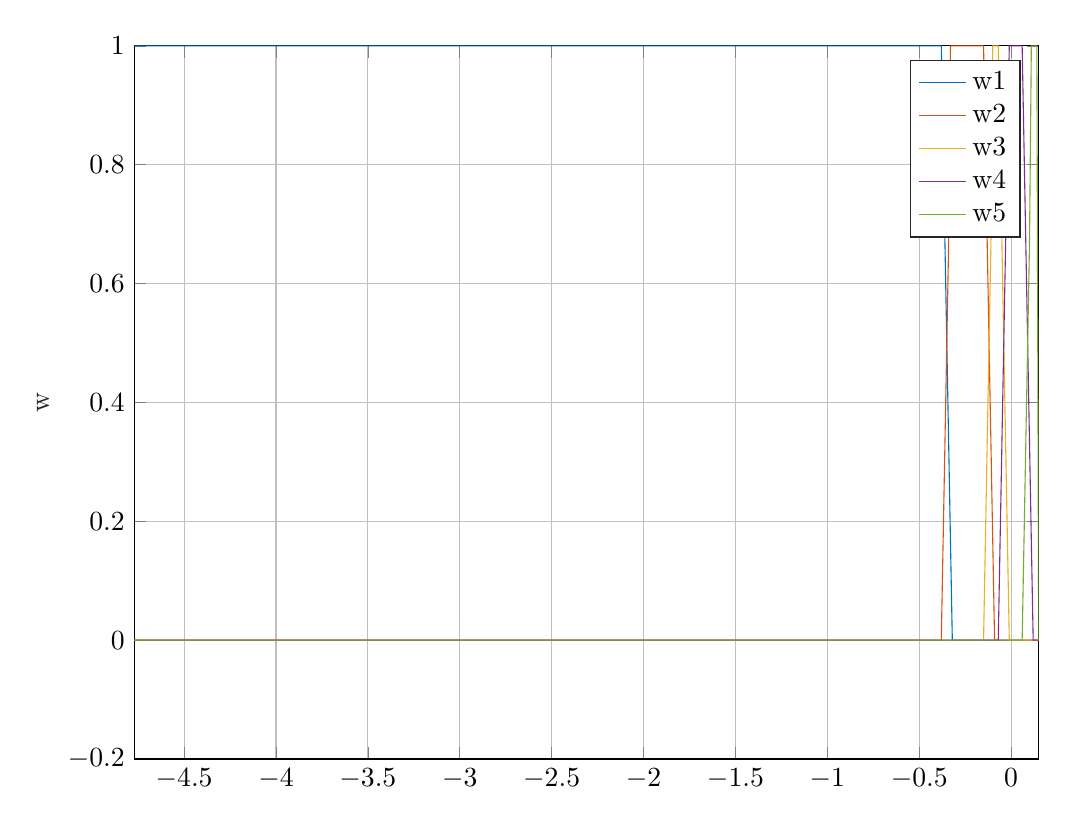
\begin{tikzpicture}

\begin{axis}[%
width=4.521in,
height=3.566in,
at={(0.758in,0.481in)},
scale only axis,
xmin=-4.77,
xmax=0.15,
ymin=-0.2,
ymax=1,
ylabel style={font=\color{white!15!black}},
ylabel={w},
axis background/.style={fill=white},
xmajorgrids,
ymajorgrids,
legend style={legend cell align=left, align=left, draw=white!15!black}
]
\addplot [color=mycolor1]
  table[row sep=crcr]{%
-4.77	1\\
-4.76	1\\
-4.75	1\\
-4.74	1\\
-4.73	1\\
-4.72	1\\
-4.71	1\\
-4.7	1\\
-4.69	1\\
-4.68	1\\
-4.67	1\\
-4.66	1\\
-4.65	1\\
-4.64	1\\
-4.63	1\\
-4.62	1\\
-4.61	1\\
-4.6	1\\
-4.59	1\\
-4.58	1\\
-4.57	1\\
-4.56	1\\
-4.55	1\\
-4.54	1\\
-4.53	1\\
-4.52	1\\
-4.51	1\\
-4.5	1\\
-4.49	1\\
-4.48	1\\
-4.47	1\\
-4.46	1\\
-4.45	1\\
-4.44	1\\
-4.43	1\\
-4.42	1\\
-4.41	1\\
-4.4	1\\
-4.39	1\\
-4.38	1\\
-4.37	1\\
-4.36	1\\
-4.35	1\\
-4.34	1\\
-4.33	1\\
-4.32	1\\
-4.31	1\\
-4.3	1\\
-4.29	1\\
-4.28	1\\
-4.27	1\\
-4.26	1\\
-4.25	1\\
-4.24	1\\
-4.23	1\\
-4.22	1\\
-4.21	1\\
-4.2	1\\
-4.19	1\\
-4.18	1\\
-4.17	1\\
-4.16	1\\
-4.15	1\\
-4.14	1\\
-4.13	1\\
-4.12	1\\
-4.11	1\\
-4.1	1\\
-4.09	1\\
-4.08	1\\
-4.07	1\\
-4.06	1\\
-4.05	1\\
-4.04	1\\
-4.03	1\\
-4.02	1\\
-4.01	1\\
-4	1\\
-3.99	1\\
-3.98	1\\
-3.97	1\\
-3.96	1\\
-3.95	1\\
-3.94	1\\
-3.93	1\\
-3.92	1\\
-3.91	1\\
-3.9	1\\
-3.89	1\\
-3.88	1\\
-3.87	1\\
-3.86	1\\
-3.85	1\\
-3.84	1\\
-3.83	1\\
-3.82	1\\
-3.81	1\\
-3.8	1\\
-3.79	1\\
-3.78	1\\
-3.77	1\\
-3.76	1\\
-3.75	1\\
-3.74	1\\
-3.73	1\\
-3.72	1\\
-3.71	1\\
-3.7	1\\
-3.69	1\\
-3.68	1\\
-3.67	1\\
-3.66	1\\
-3.65	1\\
-3.64	1\\
-3.63	1\\
-3.62	1\\
-3.61	1\\
-3.6	1\\
-3.59	1\\
-3.58	1\\
-3.57	1\\
-3.56	1\\
-3.55	1\\
-3.54	1\\
-3.53	1\\
-3.52	1\\
-3.51	1\\
-3.5	1\\
-3.49	1\\
-3.48	1\\
-3.47	1\\
-3.46	1\\
-3.45	1\\
-3.44	1\\
-3.43	1\\
-3.42	1\\
-3.41	1\\
-3.4	1\\
-3.39	1\\
-3.38	1\\
-3.37	1\\
-3.36	1\\
-3.35	1\\
-3.34	1\\
-3.33	1\\
-3.32	1\\
-3.31	1\\
-3.3	1\\
-3.29	1\\
-3.28	1\\
-3.27	1\\
-3.26	1\\
-3.25	1\\
-3.24	1\\
-3.23	1\\
-3.22	1\\
-3.21	1\\
-3.2	1\\
-3.19	1\\
-3.18	1\\
-3.17	1\\
-3.16	1\\
-3.15	1\\
-3.14	1\\
-3.13	1\\
-3.12	1\\
-3.11	1\\
-3.1	1\\
-3.09	1\\
-3.08	1\\
-3.07	1\\
-3.06	1\\
-3.05	1\\
-3.04	1\\
-3.03	1\\
-3.02	1\\
-3.01	1\\
-3	1\\
-2.99	1\\
-2.98	1\\
-2.97	1\\
-2.96	1\\
-2.95	1\\
-2.94	1\\
-2.93	1\\
-2.92	1\\
-2.91	1\\
-2.9	1\\
-2.89	1\\
-2.88	1\\
-2.87	1\\
-2.86	1\\
-2.85	1\\
-2.84	1\\
-2.83	1\\
-2.82	1\\
-2.81	1\\
-2.8	1\\
-2.79	1\\
-2.78	1\\
-2.77	1\\
-2.76	1\\
-2.75	1\\
-2.74	1\\
-2.73	1\\
-2.72	1\\
-2.71	1\\
-2.7	1\\
-2.69	1\\
-2.68	1\\
-2.67	1\\
-2.66	1\\
-2.65	1\\
-2.64	1\\
-2.63	1\\
-2.62	1\\
-2.61	1\\
-2.6	1\\
-2.59	1\\
-2.58	1\\
-2.57	1\\
-2.56	1\\
-2.55	1\\
-2.54	1\\
-2.53	1\\
-2.52	1\\
-2.51	1\\
-2.5	1\\
-2.49	1\\
-2.48	1\\
-2.47	1\\
-2.46	1\\
-2.45	1\\
-2.44	1\\
-2.43	1\\
-2.42	1\\
-2.41	1\\
-2.4	1\\
-2.39	1\\
-2.38	1\\
-2.37	1\\
-2.36	1\\
-2.35	1\\
-2.34	1\\
-2.33	1\\
-2.32	1\\
-2.31	1\\
-2.3	1\\
-2.29	1\\
-2.28	1\\
-2.27	1\\
-2.26	1\\
-2.25	1\\
-2.24	1\\
-2.23	1\\
-2.22	1\\
-2.21	1\\
-2.2	1\\
-2.19	1\\
-2.18	1\\
-2.17	1\\
-2.16	1\\
-2.15	1\\
-2.14	1\\
-2.13	1\\
-2.12	1\\
-2.11	1\\
-2.1	1\\
-2.09	1\\
-2.08	1\\
-2.07	1\\
-2.06	1\\
-2.05	1\\
-2.04	1\\
-2.03	1\\
-2.02	1\\
-2.01	1\\
-2	1\\
-1.99	1\\
-1.98	1\\
-1.97	1\\
-1.96	1\\
-1.95	1\\
-1.94	1\\
-1.93	1\\
-1.92	1\\
-1.91	1\\
-1.9	1\\
-1.89	1\\
-1.88	1\\
-1.87	1\\
-1.86	1\\
-1.85	1\\
-1.84	1\\
-1.83	1\\
-1.82	1\\
-1.81	1\\
-1.8	1\\
-1.79	1\\
-1.78	1\\
-1.77	1\\
-1.76	1\\
-1.75	1\\
-1.74	1\\
-1.73	1\\
-1.72	1\\
-1.71	1\\
-1.7	1\\
-1.69	1\\
-1.68	1\\
-1.67	1\\
-1.66	1\\
-1.65	1\\
-1.64	1\\
-1.63	1\\
-1.62	1\\
-1.61	1\\
-1.6	1\\
-1.59	1\\
-1.58	1\\
-1.57	1\\
-1.56	1\\
-1.55	1\\
-1.54	1\\
-1.53	1\\
-1.52	1\\
-1.51	1\\
-1.5	1\\
-1.49	1\\
-1.48	1\\
-1.47	1\\
-1.46	1\\
-1.45	1\\
-1.44	1\\
-1.43	1\\
-1.42	1\\
-1.41	1\\
-1.4	1\\
-1.39	1\\
-1.38	1\\
-1.37	1\\
-1.36	1\\
-1.35	1\\
-1.34	1\\
-1.33	1\\
-1.32	1\\
-1.31	1\\
-1.3	1\\
-1.29	1\\
-1.28	1\\
-1.27	1\\
-1.26	1\\
-1.25	1\\
-1.24	1\\
-1.23	1\\
-1.22	1\\
-1.21	1\\
-1.2	1\\
-1.19	1\\
-1.18	1\\
-1.17	1\\
-1.16	1\\
-1.15	1\\
-1.14	1\\
-1.13	1\\
-1.12	1\\
-1.11	1\\
-1.1	1\\
-1.09	1\\
-1.08	1\\
-1.07	1\\
-1.06	1\\
-1.05	1\\
-1.04	1\\
-1.03	1\\
-1.02	1\\
-1.01	1\\
-1	1\\
-0.99	1\\
-0.98	1\\
-0.97	1\\
-0.96	1\\
-0.95	1\\
-0.94	1\\
-0.93	1\\
-0.92	1\\
-0.91	1\\
-0.9	1\\
-0.89	1\\
-0.88	1\\
-0.87	1\\
-0.86	1\\
-0.85	1\\
-0.84	1\\
-0.83	1\\
-0.82	1\\
-0.81	1\\
-0.8	1\\
-0.79	1\\
-0.78	1\\
-0.77	1\\
-0.76	1\\
-0.75	1\\
-0.74	1\\
-0.73	1\\
-0.72	1\\
-0.71	1\\
-0.7	1\\
-0.69	1\\
-0.68	1\\
-0.67	1\\
-0.66	1\\
-0.65	1\\
-0.64	1\\
-0.63	1\\
-0.62	1\\
-0.61	1\\
-0.6	1\\
-0.59	1\\
-0.58	1\\
-0.57	1\\
-0.56	1\\
-0.55	1\\
-0.54	1\\
-0.53	1\\
-0.52	1\\
-0.51	1\\
-0.5	1\\
-0.49	1\\
-0.48	1\\
-0.47	1\\
-0.46	1\\
-0.45	1\\
-0.44	1\\
-0.43	1\\
-0.42	1\\
-0.41	1\\
-0.4	1\\
-0.39	1\\
-0.38	1\\
-0.37	0.8333\\
-0.36	0.6666\\
-0.35	0.4999\\
-0.34	0.3332\\
-0.33	0.1665\\
-0.32	0\\
-0.31	0\\
-0.3	0\\
-0.29	0\\
-0.28	0\\
-0.27	0\\
-0.26	0\\
-0.25	0\\
-0.24	0\\
-0.23	0\\
-0.22	0\\
-0.21	0\\
-0.2	0\\
-0.19	0\\
-0.18	0\\
-0.17	0\\
-0.16	0\\
-0.15	0\\
-0.14	0\\
-0.13	0\\
-0.12	0\\
-0.11	0\\
-0.1	0\\
-0.09	0\\
-0.08	0\\
-0.07	0\\
-0.06	0\\
-0.05	0\\
-0.04	0\\
-0.03	0\\
-0.02	0\\
-0.01	0\\
0	0\\
0.01	0\\
0.02	0\\
0.03	0\\
0.04	0\\
0.05	0\\
0.06	0\\
0.07	0\\
0.08	0\\
0.09	0\\
0.1	0\\
0.11	0\\
0.12	0\\
0.13	0\\
0.14	0\\
0.15	0\\
};
\addlegendentry{w1}

\addplot [color=mycolor2]
  table[row sep=crcr]{%
-4.77	0\\
-4.76	0\\
-4.75	0\\
-4.74	0\\
-4.73	0\\
-4.72	0\\
-4.71	0\\
-4.7	0\\
-4.69	0\\
-4.68	0\\
-4.67	0\\
-4.66	0\\
-4.65	0\\
-4.64	0\\
-4.63	0\\
-4.62	0\\
-4.61	0\\
-4.6	0\\
-4.59	0\\
-4.58	0\\
-4.57	0\\
-4.56	0\\
-4.55	0\\
-4.54	0\\
-4.53	0\\
-4.52	0\\
-4.51	0\\
-4.5	0\\
-4.49	0\\
-4.48	0\\
-4.47	0\\
-4.46	0\\
-4.45	0\\
-4.44	0\\
-4.43	0\\
-4.42	0\\
-4.41	0\\
-4.4	0\\
-4.39	0\\
-4.38	0\\
-4.37	0\\
-4.36	0\\
-4.35	0\\
-4.34	0\\
-4.33	0\\
-4.32	0\\
-4.31	0\\
-4.3	0\\
-4.29	0\\
-4.28	0\\
-4.27	0\\
-4.26	0\\
-4.25	0\\
-4.24	0\\
-4.23	0\\
-4.22	0\\
-4.21	0\\
-4.2	0\\
-4.19	0\\
-4.18	0\\
-4.17	0\\
-4.16	0\\
-4.15	0\\
-4.14	0\\
-4.13	0\\
-4.12	0\\
-4.11	0\\
-4.1	0\\
-4.09	0\\
-4.08	0\\
-4.07	0\\
-4.06	0\\
-4.05	0\\
-4.04	0\\
-4.03	0\\
-4.02	0\\
-4.01	0\\
-4	0\\
-3.99	0\\
-3.98	0\\
-3.97	0\\
-3.96	0\\
-3.95	0\\
-3.94	0\\
-3.93	0\\
-3.92	0\\
-3.91	0\\
-3.9	0\\
-3.89	0\\
-3.88	0\\
-3.87	0\\
-3.86	0\\
-3.85	0\\
-3.84	0\\
-3.83	0\\
-3.82	0\\
-3.81	0\\
-3.8	0\\
-3.79	0\\
-3.78	0\\
-3.77	0\\
-3.76	0\\
-3.75	0\\
-3.74	0\\
-3.73	0\\
-3.72	0\\
-3.71	0\\
-3.7	0\\
-3.69	0\\
-3.68	0\\
-3.67	0\\
-3.66	0\\
-3.65	0\\
-3.64	0\\
-3.63	0\\
-3.62	0\\
-3.61	0\\
-3.6	0\\
-3.59	0\\
-3.58	0\\
-3.57	0\\
-3.56	0\\
-3.55	0\\
-3.54	0\\
-3.53	0\\
-3.52	0\\
-3.51	0\\
-3.5	0\\
-3.49	0\\
-3.48	0\\
-3.47	0\\
-3.46	0\\
-3.45	0\\
-3.44	0\\
-3.43	0\\
-3.42	0\\
-3.41	0\\
-3.4	0\\
-3.39	0\\
-3.38	0\\
-3.37	0\\
-3.36	0\\
-3.35	0\\
-3.34	0\\
-3.33	0\\
-3.32	0\\
-3.31	0\\
-3.3	0\\
-3.29	0\\
-3.28	0\\
-3.27	0\\
-3.26	0\\
-3.25	0\\
-3.24	0\\
-3.23	0\\
-3.22	0\\
-3.21	0\\
-3.2	0\\
-3.19	0\\
-3.18	0\\
-3.17	0\\
-3.16	0\\
-3.15	0\\
-3.14	0\\
-3.13	0\\
-3.12	0\\
-3.11	0\\
-3.1	0\\
-3.09	0\\
-3.08	0\\
-3.07	0\\
-3.06	0\\
-3.05	0\\
-3.04	0\\
-3.03	0\\
-3.02	0\\
-3.01	0\\
-3	0\\
-2.99	0\\
-2.98	0\\
-2.97	0\\
-2.96	0\\
-2.95	0\\
-2.94	0\\
-2.93	0\\
-2.92	0\\
-2.91	0\\
-2.9	0\\
-2.89	0\\
-2.88	0\\
-2.87	0\\
-2.86	0\\
-2.85	0\\
-2.84	0\\
-2.83	0\\
-2.82	0\\
-2.81	0\\
-2.8	0\\
-2.79	0\\
-2.78	0\\
-2.77	0\\
-2.76	0\\
-2.75	0\\
-2.74	0\\
-2.73	0\\
-2.72	0\\
-2.71	0\\
-2.7	0\\
-2.69	0\\
-2.68	0\\
-2.67	0\\
-2.66	0\\
-2.65	0\\
-2.64	0\\
-2.63	0\\
-2.62	0\\
-2.61	0\\
-2.6	0\\
-2.59	0\\
-2.58	0\\
-2.57	0\\
-2.56	0\\
-2.55	0\\
-2.54	0\\
-2.53	0\\
-2.52	0\\
-2.51	0\\
-2.5	0\\
-2.49	0\\
-2.48	0\\
-2.47	0\\
-2.46	0\\
-2.45	0\\
-2.44	0\\
-2.43	0\\
-2.42	0\\
-2.41	0\\
-2.4	0\\
-2.39	0\\
-2.38	0\\
-2.37	0\\
-2.36	0\\
-2.35	0\\
-2.34	0\\
-2.33	0\\
-2.32	0\\
-2.31	0\\
-2.3	0\\
-2.29	0\\
-2.28	0\\
-2.27	0\\
-2.26	0\\
-2.25	0\\
-2.24	0\\
-2.23	0\\
-2.22	0\\
-2.21	0\\
-2.2	0\\
-2.19	0\\
-2.18	0\\
-2.17	0\\
-2.16	0\\
-2.15	0\\
-2.14	0\\
-2.13	0\\
-2.12	0\\
-2.11	0\\
-2.1	0\\
-2.09	0\\
-2.08	0\\
-2.07	0\\
-2.06	0\\
-2.05	0\\
-2.04	0\\
-2.03	0\\
-2.02	0\\
-2.01	0\\
-2	0\\
-1.99	0\\
-1.98	0\\
-1.97	0\\
-1.96	0\\
-1.95	0\\
-1.94	0\\
-1.93	0\\
-1.92	0\\
-1.91	0\\
-1.9	0\\
-1.89	0\\
-1.88	0\\
-1.87	0\\
-1.86	0\\
-1.85	0\\
-1.84	0\\
-1.83	0\\
-1.82	0\\
-1.81	0\\
-1.8	0\\
-1.79	0\\
-1.78	0\\
-1.77	0\\
-1.76	0\\
-1.75	0\\
-1.74	0\\
-1.73	0\\
-1.72	0\\
-1.71	0\\
-1.7	0\\
-1.69	0\\
-1.68	0\\
-1.67	0\\
-1.66	0\\
-1.65	0\\
-1.64	0\\
-1.63	0\\
-1.62	0\\
-1.61	0\\
-1.6	0\\
-1.59	0\\
-1.58	0\\
-1.57	0\\
-1.56	0\\
-1.55	0\\
-1.54	0\\
-1.53	0\\
-1.52	0\\
-1.51	0\\
-1.5	0\\
-1.49	0\\
-1.48	0\\
-1.47	0\\
-1.46	0\\
-1.45	0\\
-1.44	0\\
-1.43	0\\
-1.42	0\\
-1.41	0\\
-1.4	0\\
-1.39	0\\
-1.38	0\\
-1.37	0\\
-1.36	0\\
-1.35	0\\
-1.34	0\\
-1.33	0\\
-1.32	0\\
-1.31	0\\
-1.3	0\\
-1.29	0\\
-1.28	0\\
-1.27	0\\
-1.26	0\\
-1.25	0\\
-1.24	0\\
-1.23	0\\
-1.22	0\\
-1.21	0\\
-1.2	0\\
-1.19	0\\
-1.18	0\\
-1.17	0\\
-1.16	0\\
-1.15	0\\
-1.14	0\\
-1.13	0\\
-1.12	0\\
-1.11	0\\
-1.1	0\\
-1.09	0\\
-1.08	0\\
-1.07	0\\
-1.06	0\\
-1.05	0\\
-1.04	0\\
-1.03	0\\
-1.02	0\\
-1.01	0\\
-1	0\\
-0.99	0\\
-0.98	0\\
-0.97	0\\
-0.96	0\\
-0.95	0\\
-0.94	0\\
-0.93	0\\
-0.92	0\\
-0.91	0\\
-0.9	0\\
-0.89	0\\
-0.88	0\\
-0.87	0\\
-0.86	0\\
-0.85	0\\
-0.84	0\\
-0.83	0\\
-0.82	0\\
-0.81	0\\
-0.8	0\\
-0.79	0\\
-0.78	0\\
-0.77	0\\
-0.76	0\\
-0.75	0\\
-0.74	0\\
-0.73	0\\
-0.72	0\\
-0.71	0\\
-0.7	0\\
-0.69	0\\
-0.68	0\\
-0.67	0\\
-0.66	0\\
-0.65	0\\
-0.64	0\\
-0.63	0\\
-0.62	0\\
-0.61	0\\
-0.6	0\\
-0.59	0\\
-0.58	0\\
-0.57	0\\
-0.56	0\\
-0.55	0\\
-0.54	0\\
-0.53	0\\
-0.52	0\\
-0.51	0\\
-0.5	0\\
-0.49	0\\
-0.48	0\\
-0.47	0\\
-0.46	0\\
-0.45	0\\
-0.44	0\\
-0.43	0\\
-0.42	0\\
-0.41	0\\
-0.4	0\\
-0.39	0\\
-0.38	-8.8818e-16\\
-0.37	0.1667\\
-0.36	0.3334\\
-0.35	0.5001\\
-0.34	0.6668\\
-0.33	1\\
-0.32	1\\
-0.31	1\\
-0.3	1\\
-0.29	1\\
-0.28	1\\
-0.27	1\\
-0.26	1\\
-0.25	1\\
-0.24	1\\
-0.23	1\\
-0.22	1\\
-0.21	1\\
-0.2	1\\
-0.19	1\\
-0.18	1\\
-0.17	1\\
-0.16	1\\
-0.15	1\\
-0.14	0.8333\\
-0.13	0.6666\\
-0.12	0.4999\\
-0.11	0.3332\\
-0.1	0.1665\\
-0.09	0\\
-0.08	0\\
-0.07	0\\
-0.06	0\\
-0.05	0\\
-0.04	0\\
-0.03	0\\
-0.02	0\\
-0.01	0\\
0	0\\
0.01	0\\
0.02	0\\
0.03	0\\
0.04	0\\
0.05	0\\
0.06	0\\
0.07	0\\
0.08	0\\
0.09	0\\
0.1	0\\
0.11	0\\
0.12	0\\
0.13	0\\
0.14	0\\
0.15	0\\
};
\addlegendentry{w2}

\addplot [color=mycolor3]
  table[row sep=crcr]{%
-4.77	0\\
-4.76	0\\
-4.75	0\\
-4.74	0\\
-4.73	0\\
-4.72	0\\
-4.71	0\\
-4.7	0\\
-4.69	0\\
-4.68	0\\
-4.67	0\\
-4.66	0\\
-4.65	0\\
-4.64	0\\
-4.63	0\\
-4.62	0\\
-4.61	0\\
-4.6	0\\
-4.59	0\\
-4.58	0\\
-4.57	0\\
-4.56	0\\
-4.55	0\\
-4.54	0\\
-4.53	0\\
-4.52	0\\
-4.51	0\\
-4.5	0\\
-4.49	0\\
-4.48	0\\
-4.47	0\\
-4.46	0\\
-4.45	0\\
-4.44	0\\
-4.43	0\\
-4.42	0\\
-4.41	0\\
-4.4	0\\
-4.39	0\\
-4.38	0\\
-4.37	0\\
-4.36	0\\
-4.35	0\\
-4.34	0\\
-4.33	0\\
-4.32	0\\
-4.31	0\\
-4.3	0\\
-4.29	0\\
-4.28	0\\
-4.27	0\\
-4.26	0\\
-4.25	0\\
-4.24	0\\
-4.23	0\\
-4.22	0\\
-4.21	0\\
-4.2	0\\
-4.19	0\\
-4.18	0\\
-4.17	0\\
-4.16	0\\
-4.15	0\\
-4.14	0\\
-4.13	0\\
-4.12	0\\
-4.11	0\\
-4.1	0\\
-4.09	0\\
-4.08	0\\
-4.07	0\\
-4.06	0\\
-4.05	0\\
-4.04	0\\
-4.03	0\\
-4.02	0\\
-4.01	0\\
-4	0\\
-3.99	0\\
-3.98	0\\
-3.97	0\\
-3.96	0\\
-3.95	0\\
-3.94	0\\
-3.93	0\\
-3.92	0\\
-3.91	0\\
-3.9	0\\
-3.89	0\\
-3.88	0\\
-3.87	0\\
-3.86	0\\
-3.85	0\\
-3.84	0\\
-3.83	0\\
-3.82	0\\
-3.81	0\\
-3.8	0\\
-3.79	0\\
-3.78	0\\
-3.77	0\\
-3.76	0\\
-3.75	0\\
-3.74	0\\
-3.73	0\\
-3.72	0\\
-3.71	0\\
-3.7	0\\
-3.69	0\\
-3.68	0\\
-3.67	0\\
-3.66	0\\
-3.65	0\\
-3.64	0\\
-3.63	0\\
-3.62	0\\
-3.61	0\\
-3.6	0\\
-3.59	0\\
-3.58	0\\
-3.57	0\\
-3.56	0\\
-3.55	0\\
-3.54	0\\
-3.53	0\\
-3.52	0\\
-3.51	0\\
-3.5	0\\
-3.49	0\\
-3.48	0\\
-3.47	0\\
-3.46	0\\
-3.45	0\\
-3.44	0\\
-3.43	0\\
-3.42	0\\
-3.41	0\\
-3.4	0\\
-3.39	0\\
-3.38	0\\
-3.37	0\\
-3.36	0\\
-3.35	0\\
-3.34	0\\
-3.33	0\\
-3.32	0\\
-3.31	0\\
-3.3	0\\
-3.29	0\\
-3.28	0\\
-3.27	0\\
-3.26	0\\
-3.25	0\\
-3.24	0\\
-3.23	0\\
-3.22	0\\
-3.21	0\\
-3.2	0\\
-3.19	0\\
-3.18	0\\
-3.17	0\\
-3.16	0\\
-3.15	0\\
-3.14	0\\
-3.13	0\\
-3.12	0\\
-3.11	0\\
-3.1	0\\
-3.09	0\\
-3.08	0\\
-3.07	0\\
-3.06	0\\
-3.05	0\\
-3.04	0\\
-3.03	0\\
-3.02	0\\
-3.01	0\\
-3	0\\
-2.99	0\\
-2.98	0\\
-2.97	0\\
-2.96	0\\
-2.95	0\\
-2.94	0\\
-2.93	0\\
-2.92	0\\
-2.91	0\\
-2.9	0\\
-2.89	0\\
-2.88	0\\
-2.87	0\\
-2.86	0\\
-2.85	0\\
-2.84	0\\
-2.83	0\\
-2.82	0\\
-2.81	0\\
-2.8	0\\
-2.79	0\\
-2.78	0\\
-2.77	0\\
-2.76	0\\
-2.75	0\\
-2.74	0\\
-2.73	0\\
-2.72	0\\
-2.71	0\\
-2.7	0\\
-2.69	0\\
-2.68	0\\
-2.67	0\\
-2.66	0\\
-2.65	0\\
-2.64	0\\
-2.63	0\\
-2.62	0\\
-2.61	0\\
-2.6	0\\
-2.59	0\\
-2.58	0\\
-2.57	0\\
-2.56	0\\
-2.55	0\\
-2.54	0\\
-2.53	0\\
-2.52	0\\
-2.51	0\\
-2.5	0\\
-2.49	0\\
-2.48	0\\
-2.47	0\\
-2.46	0\\
-2.45	0\\
-2.44	0\\
-2.43	0\\
-2.42	0\\
-2.41	0\\
-2.4	0\\
-2.39	0\\
-2.38	0\\
-2.37	0\\
-2.36	0\\
-2.35	0\\
-2.34	0\\
-2.33	0\\
-2.32	0\\
-2.31	0\\
-2.3	0\\
-2.29	0\\
-2.28	0\\
-2.27	0\\
-2.26	0\\
-2.25	0\\
-2.24	0\\
-2.23	0\\
-2.22	0\\
-2.21	0\\
-2.2	0\\
-2.19	0\\
-2.18	0\\
-2.17	0\\
-2.16	0\\
-2.15	0\\
-2.14	0\\
-2.13	0\\
-2.12	0\\
-2.11	0\\
-2.1	0\\
-2.09	0\\
-2.08	0\\
-2.07	0\\
-2.06	0\\
-2.05	0\\
-2.04	0\\
-2.03	0\\
-2.02	0\\
-2.01	0\\
-2	0\\
-1.99	0\\
-1.98	0\\
-1.97	0\\
-1.96	0\\
-1.95	0\\
-1.94	0\\
-1.93	0\\
-1.92	0\\
-1.91	0\\
-1.9	0\\
-1.89	0\\
-1.88	0\\
-1.87	0\\
-1.86	0\\
-1.85	0\\
-1.84	0\\
-1.83	0\\
-1.82	0\\
-1.81	0\\
-1.8	0\\
-1.79	0\\
-1.78	0\\
-1.77	0\\
-1.76	0\\
-1.75	0\\
-1.74	0\\
-1.73	0\\
-1.72	0\\
-1.71	0\\
-1.7	0\\
-1.69	0\\
-1.68	0\\
-1.67	0\\
-1.66	0\\
-1.65	0\\
-1.64	0\\
-1.63	0\\
-1.62	0\\
-1.61	0\\
-1.6	0\\
-1.59	0\\
-1.58	0\\
-1.57	0\\
-1.56	0\\
-1.55	0\\
-1.54	0\\
-1.53	0\\
-1.52	0\\
-1.51	0\\
-1.5	0\\
-1.49	0\\
-1.48	0\\
-1.47	0\\
-1.46	0\\
-1.45	0\\
-1.44	0\\
-1.43	0\\
-1.42	0\\
-1.41	0\\
-1.4	0\\
-1.39	0\\
-1.38	0\\
-1.37	0\\
-1.36	0\\
-1.35	0\\
-1.34	0\\
-1.33	0\\
-1.32	0\\
-1.31	0\\
-1.3	0\\
-1.29	0\\
-1.28	0\\
-1.27	0\\
-1.26	0\\
-1.25	0\\
-1.24	0\\
-1.23	0\\
-1.22	0\\
-1.21	0\\
-1.2	0\\
-1.19	0\\
-1.18	0\\
-1.17	0\\
-1.16	0\\
-1.15	0\\
-1.14	0\\
-1.13	0\\
-1.12	0\\
-1.11	0\\
-1.1	0\\
-1.09	0\\
-1.08	0\\
-1.07	0\\
-1.06	0\\
-1.05	0\\
-1.04	0\\
-1.03	0\\
-1.02	0\\
-1.01	0\\
-1	0\\
-0.99	0\\
-0.98	0\\
-0.97	0\\
-0.96	0\\
-0.95	0\\
-0.94	0\\
-0.93	0\\
-0.92	0\\
-0.91	0\\
-0.9	0\\
-0.89	0\\
-0.88	0\\
-0.87	0\\
-0.86	0\\
-0.85	0\\
-0.84	0\\
-0.83	0\\
-0.82	0\\
-0.81	0\\
-0.8	0\\
-0.79	0\\
-0.78	0\\
-0.77	0\\
-0.76	0\\
-0.75	0\\
-0.74	0\\
-0.73	0\\
-0.72	0\\
-0.71	0\\
-0.7	0\\
-0.69	0\\
-0.68	0\\
-0.67	0\\
-0.66	0\\
-0.65	0\\
-0.64	0\\
-0.63	0\\
-0.62	0\\
-0.61	0\\
-0.6	0\\
-0.59	0\\
-0.58	0\\
-0.57	0\\
-0.56	0\\
-0.55	0\\
-0.54	0\\
-0.53	0\\
-0.52	0\\
-0.51	0\\
-0.5	0\\
-0.49	0\\
-0.48	0\\
-0.47	0\\
-0.46	0\\
-0.45	0\\
-0.44	0\\
-0.43	0\\
-0.42	0\\
-0.41	0\\
-0.4	0\\
-0.39	0\\
-0.38	0\\
-0.37	0\\
-0.36	0\\
-0.35	0\\
-0.34	0\\
-0.33	0\\
-0.32	0\\
-0.31	0\\
-0.3	0\\
-0.29	0\\
-0.28	0\\
-0.27	0\\
-0.26	0\\
-0.25	0\\
-0.24	0\\
-0.23	0\\
-0.22	0\\
-0.21	0\\
-0.2	0\\
-0.19	0\\
-0.18	0\\
-0.17	0\\
-0.16	0\\
-0.15	0\\
-0.14	0.1667\\
-0.13	0.3334\\
-0.12	0.5001\\
-0.11	0.6668\\
-0.1	1\\
-0.09	1\\
-0.08	1\\
-0.07	1\\
-0.06	0.8333\\
-0.05	0.6666\\
-0.04	0.4999\\
-0.03	0.3332\\
-0.02	0.1665\\
-0.01	-0.0002\\
0	0\\
0.01	0\\
0.02	0\\
0.03	0\\
0.04	0\\
0.05	0\\
0.06	0\\
0.07	0\\
0.08	0\\
0.09	0\\
0.1	0\\
0.11	0\\
0.12	0\\
0.13	0\\
0.14	0\\
0.15	0\\
};
\addlegendentry{w3}

\addplot [color=mycolor4]
  table[row sep=crcr]{%
-4.77	0\\
-4.76	0\\
-4.75	0\\
-4.74	0\\
-4.73	0\\
-4.72	0\\
-4.71	0\\
-4.7	0\\
-4.69	0\\
-4.68	0\\
-4.67	0\\
-4.66	0\\
-4.65	0\\
-4.64	0\\
-4.63	0\\
-4.62	0\\
-4.61	0\\
-4.6	0\\
-4.59	0\\
-4.58	0\\
-4.57	0\\
-4.56	0\\
-4.55	0\\
-4.54	0\\
-4.53	0\\
-4.52	0\\
-4.51	0\\
-4.5	0\\
-4.49	0\\
-4.48	0\\
-4.47	0\\
-4.46	0\\
-4.45	0\\
-4.44	0\\
-4.43	0\\
-4.42	0\\
-4.41	0\\
-4.4	0\\
-4.39	0\\
-4.38	0\\
-4.37	0\\
-4.36	0\\
-4.35	0\\
-4.34	0\\
-4.33	0\\
-4.32	0\\
-4.31	0\\
-4.3	0\\
-4.29	0\\
-4.28	0\\
-4.27	0\\
-4.26	0\\
-4.25	0\\
-4.24	0\\
-4.23	0\\
-4.22	0\\
-4.21	0\\
-4.2	0\\
-4.19	0\\
-4.18	0\\
-4.17	0\\
-4.16	0\\
-4.15	0\\
-4.14	0\\
-4.13	0\\
-4.12	0\\
-4.11	0\\
-4.1	0\\
-4.09	0\\
-4.08	0\\
-4.07	0\\
-4.06	0\\
-4.05	0\\
-4.04	0\\
-4.03	0\\
-4.02	0\\
-4.01	0\\
-4	0\\
-3.99	0\\
-3.98	0\\
-3.97	0\\
-3.96	0\\
-3.95	0\\
-3.94	0\\
-3.93	0\\
-3.92	0\\
-3.91	0\\
-3.9	0\\
-3.89	0\\
-3.88	0\\
-3.87	0\\
-3.86	0\\
-3.85	0\\
-3.84	0\\
-3.83	0\\
-3.82	0\\
-3.81	0\\
-3.8	0\\
-3.79	0\\
-3.78	0\\
-3.77	0\\
-3.76	0\\
-3.75	0\\
-3.74	0\\
-3.73	0\\
-3.72	0\\
-3.71	0\\
-3.7	0\\
-3.69	0\\
-3.68	0\\
-3.67	0\\
-3.66	0\\
-3.65	0\\
-3.64	0\\
-3.63	0\\
-3.62	0\\
-3.61	0\\
-3.6	0\\
-3.59	0\\
-3.58	0\\
-3.57	0\\
-3.56	0\\
-3.55	0\\
-3.54	0\\
-3.53	0\\
-3.52	0\\
-3.51	0\\
-3.5	0\\
-3.49	0\\
-3.48	0\\
-3.47	0\\
-3.46	0\\
-3.45	0\\
-3.44	0\\
-3.43	0\\
-3.42	0\\
-3.41	0\\
-3.4	0\\
-3.39	0\\
-3.38	0\\
-3.37	0\\
-3.36	0\\
-3.35	0\\
-3.34	0\\
-3.33	0\\
-3.32	0\\
-3.31	0\\
-3.3	0\\
-3.29	0\\
-3.28	0\\
-3.27	0\\
-3.26	0\\
-3.25	0\\
-3.24	0\\
-3.23	0\\
-3.22	0\\
-3.21	0\\
-3.2	0\\
-3.19	0\\
-3.18	0\\
-3.17	0\\
-3.16	0\\
-3.15	0\\
-3.14	0\\
-3.13	0\\
-3.12	0\\
-3.11	0\\
-3.1	0\\
-3.09	0\\
-3.08	0\\
-3.07	0\\
-3.06	0\\
-3.05	0\\
-3.04	0\\
-3.03	0\\
-3.02	0\\
-3.01	0\\
-3	0\\
-2.99	0\\
-2.98	0\\
-2.97	0\\
-2.96	0\\
-2.95	0\\
-2.94	0\\
-2.93	0\\
-2.92	0\\
-2.91	0\\
-2.9	0\\
-2.89	0\\
-2.88	0\\
-2.87	0\\
-2.86	0\\
-2.85	0\\
-2.84	0\\
-2.83	0\\
-2.82	0\\
-2.81	0\\
-2.8	0\\
-2.79	0\\
-2.78	0\\
-2.77	0\\
-2.76	0\\
-2.75	0\\
-2.74	0\\
-2.73	0\\
-2.72	0\\
-2.71	0\\
-2.7	0\\
-2.69	0\\
-2.68	0\\
-2.67	0\\
-2.66	0\\
-2.65	0\\
-2.64	0\\
-2.63	0\\
-2.62	0\\
-2.61	0\\
-2.6	0\\
-2.59	0\\
-2.58	0\\
-2.57	0\\
-2.56	0\\
-2.55	0\\
-2.54	0\\
-2.53	0\\
-2.52	0\\
-2.51	0\\
-2.5	0\\
-2.49	0\\
-2.48	0\\
-2.47	0\\
-2.46	0\\
-2.45	0\\
-2.44	0\\
-2.43	0\\
-2.42	0\\
-2.41	0\\
-2.4	0\\
-2.39	0\\
-2.38	0\\
-2.37	0\\
-2.36	0\\
-2.35	0\\
-2.34	0\\
-2.33	0\\
-2.32	0\\
-2.31	0\\
-2.3	0\\
-2.29	0\\
-2.28	0\\
-2.27	0\\
-2.26	0\\
-2.25	0\\
-2.24	0\\
-2.23	0\\
-2.22	0\\
-2.21	0\\
-2.2	0\\
-2.19	0\\
-2.18	0\\
-2.17	0\\
-2.16	0\\
-2.15	0\\
-2.14	0\\
-2.13	0\\
-2.12	0\\
-2.11	0\\
-2.1	0\\
-2.09	0\\
-2.08	0\\
-2.07	0\\
-2.06	0\\
-2.05	0\\
-2.04	0\\
-2.03	0\\
-2.02	0\\
-2.01	0\\
-2	0\\
-1.99	0\\
-1.98	0\\
-1.97	0\\
-1.96	0\\
-1.95	0\\
-1.94	0\\
-1.93	0\\
-1.92	0\\
-1.91	0\\
-1.9	0\\
-1.89	0\\
-1.88	0\\
-1.87	0\\
-1.86	0\\
-1.85	0\\
-1.84	0\\
-1.83	0\\
-1.82	0\\
-1.81	0\\
-1.8	0\\
-1.79	0\\
-1.78	0\\
-1.77	0\\
-1.76	0\\
-1.75	0\\
-1.74	0\\
-1.73	0\\
-1.72	0\\
-1.71	0\\
-1.7	0\\
-1.69	0\\
-1.68	0\\
-1.67	0\\
-1.66	0\\
-1.65	0\\
-1.64	0\\
-1.63	0\\
-1.62	0\\
-1.61	0\\
-1.6	0\\
-1.59	0\\
-1.58	0\\
-1.57	0\\
-1.56	0\\
-1.55	0\\
-1.54	0\\
-1.53	0\\
-1.52	0\\
-1.51	0\\
-1.5	0\\
-1.49	0\\
-1.48	0\\
-1.47	0\\
-1.46	0\\
-1.45	0\\
-1.44	0\\
-1.43	0\\
-1.42	0\\
-1.41	0\\
-1.4	0\\
-1.39	0\\
-1.38	0\\
-1.37	0\\
-1.36	0\\
-1.35	0\\
-1.34	0\\
-1.33	0\\
-1.32	0\\
-1.31	0\\
-1.3	0\\
-1.29	0\\
-1.28	0\\
-1.27	0\\
-1.26	0\\
-1.25	0\\
-1.24	0\\
-1.23	0\\
-1.22	0\\
-1.21	0\\
-1.2	0\\
-1.19	0\\
-1.18	0\\
-1.17	0\\
-1.16	0\\
-1.15	0\\
-1.14	0\\
-1.13	0\\
-1.12	0\\
-1.11	0\\
-1.1	0\\
-1.09	0\\
-1.08	0\\
-1.07	0\\
-1.06	0\\
-1.05	0\\
-1.04	0\\
-1.03	0\\
-1.02	0\\
-1.01	0\\
-1	0\\
-0.99	0\\
-0.98	0\\
-0.97	0\\
-0.96	0\\
-0.95	0\\
-0.94	0\\
-0.93	0\\
-0.92	0\\
-0.91	0\\
-0.9	0\\
-0.89	0\\
-0.88	0\\
-0.87	0\\
-0.86	0\\
-0.85	0\\
-0.84	0\\
-0.83	0\\
-0.82	0\\
-0.81	0\\
-0.8	0\\
-0.79	0\\
-0.78	0\\
-0.77	0\\
-0.76	0\\
-0.75	0\\
-0.74	0\\
-0.73	0\\
-0.72	0\\
-0.71	0\\
-0.7	0\\
-0.69	0\\
-0.68	0\\
-0.67	0\\
-0.66	0\\
-0.65	0\\
-0.64	0\\
-0.63	0\\
-0.62	0\\
-0.61	0\\
-0.6	0\\
-0.59	0\\
-0.58	0\\
-0.57	0\\
-0.56	0\\
-0.55	0\\
-0.54	0\\
-0.53	0\\
-0.52	0\\
-0.51	0\\
-0.5	0\\
-0.49	0\\
-0.48	0\\
-0.47	0\\
-0.46	0\\
-0.45	0\\
-0.44	0\\
-0.43	0\\
-0.42	0\\
-0.41	0\\
-0.4	0\\
-0.39	0\\
-0.38	0\\
-0.37	0\\
-0.36	0\\
-0.35	0\\
-0.34	0\\
-0.33	0\\
-0.32	0\\
-0.31	0\\
-0.3	0\\
-0.29	0\\
-0.28	0\\
-0.27	0\\
-0.26	0\\
-0.25	0\\
-0.24	0\\
-0.23	0\\
-0.22	0\\
-0.21	0\\
-0.2	0\\
-0.19	0\\
-0.18	0\\
-0.17	0\\
-0.16	0\\
-0.15	0\\
-0.14	0\\
-0.13	0\\
-0.12	0\\
-0.11	0\\
-0.1	0\\
-0.09	0\\
-0.08	0\\
-0.07	-2.2204e-16\\
-0.06	0.1667\\
-0.05	0.3334\\
-0.04	0.5001\\
-0.03	0.6668\\
-0.02	0.8335\\
-0.01	1\\
0	1\\
0.01	1\\
0.02	1\\
0.03	1\\
0.04	1\\
0.05	1\\
0.06	1\\
0.07	0.8333\\
0.08	0.6666\\
0.09	0.4999\\
0.1	0.3332\\
0.11	0.1665\\
0.12	0\\
0.13	0\\
0.14	0\\
0.15	0\\
};
\addlegendentry{w4}

\addplot [color=mycolor5]
  table[row sep=crcr]{%
-4.77	0\\
-4.76	0\\
-4.75	0\\
-4.74	0\\
-4.73	0\\
-4.72	0\\
-4.71	0\\
-4.7	0\\
-4.69	0\\
-4.68	0\\
-4.67	0\\
-4.66	0\\
-4.65	0\\
-4.64	0\\
-4.63	0\\
-4.62	0\\
-4.61	0\\
-4.6	0\\
-4.59	0\\
-4.58	0\\
-4.57	0\\
-4.56	0\\
-4.55	0\\
-4.54	0\\
-4.53	0\\
-4.52	0\\
-4.51	0\\
-4.5	0\\
-4.49	0\\
-4.48	0\\
-4.47	0\\
-4.46	0\\
-4.45	0\\
-4.44	0\\
-4.43	0\\
-4.42	0\\
-4.41	0\\
-4.4	0\\
-4.39	0\\
-4.38	0\\
-4.37	0\\
-4.36	0\\
-4.35	0\\
-4.34	0\\
-4.33	0\\
-4.32	0\\
-4.31	0\\
-4.3	0\\
-4.29	0\\
-4.28	0\\
-4.27	0\\
-4.26	0\\
-4.25	0\\
-4.24	0\\
-4.23	0\\
-4.22	0\\
-4.21	0\\
-4.2	0\\
-4.19	0\\
-4.18	0\\
-4.17	0\\
-4.16	0\\
-4.15	0\\
-4.14	0\\
-4.13	0\\
-4.12	0\\
-4.11	0\\
-4.1	0\\
-4.09	0\\
-4.08	0\\
-4.07	0\\
-4.06	0\\
-4.05	0\\
-4.04	0\\
-4.03	0\\
-4.02	0\\
-4.01	0\\
-4	0\\
-3.99	0\\
-3.98	0\\
-3.97	0\\
-3.96	0\\
-3.95	0\\
-3.94	0\\
-3.93	0\\
-3.92	0\\
-3.91	0\\
-3.9	0\\
-3.89	0\\
-3.88	0\\
-3.87	0\\
-3.86	0\\
-3.85	0\\
-3.84	0\\
-3.83	0\\
-3.82	0\\
-3.81	0\\
-3.8	0\\
-3.79	0\\
-3.78	0\\
-3.77	0\\
-3.76	0\\
-3.75	0\\
-3.74	0\\
-3.73	0\\
-3.72	0\\
-3.71	0\\
-3.7	0\\
-3.69	0\\
-3.68	0\\
-3.67	0\\
-3.66	0\\
-3.65	0\\
-3.64	0\\
-3.63	0\\
-3.62	0\\
-3.61	0\\
-3.6	0\\
-3.59	0\\
-3.58	0\\
-3.57	0\\
-3.56	0\\
-3.55	0\\
-3.54	0\\
-3.53	0\\
-3.52	0\\
-3.51	0\\
-3.5	0\\
-3.49	0\\
-3.48	0\\
-3.47	0\\
-3.46	0\\
-3.45	0\\
-3.44	0\\
-3.43	0\\
-3.42	0\\
-3.41	0\\
-3.4	0\\
-3.39	0\\
-3.38	0\\
-3.37	0\\
-3.36	0\\
-3.35	0\\
-3.34	0\\
-3.33	0\\
-3.32	0\\
-3.31	0\\
-3.3	0\\
-3.29	0\\
-3.28	0\\
-3.27	0\\
-3.26	0\\
-3.25	0\\
-3.24	0\\
-3.23	0\\
-3.22	0\\
-3.21	0\\
-3.2	0\\
-3.19	0\\
-3.18	0\\
-3.17	0\\
-3.16	0\\
-3.15	0\\
-3.14	0\\
-3.13	0\\
-3.12	0\\
-3.11	0\\
-3.1	0\\
-3.09	0\\
-3.08	0\\
-3.07	0\\
-3.06	0\\
-3.05	0\\
-3.04	0\\
-3.03	0\\
-3.02	0\\
-3.01	0\\
-3	0\\
-2.99	0\\
-2.98	0\\
-2.97	0\\
-2.96	0\\
-2.95	0\\
-2.94	0\\
-2.93	0\\
-2.92	0\\
-2.91	0\\
-2.9	0\\
-2.89	0\\
-2.88	0\\
-2.87	0\\
-2.86	0\\
-2.85	0\\
-2.84	0\\
-2.83	0\\
-2.82	0\\
-2.81	0\\
-2.8	0\\
-2.79	0\\
-2.78	0\\
-2.77	0\\
-2.76	0\\
-2.75	0\\
-2.74	0\\
-2.73	0\\
-2.72	0\\
-2.71	0\\
-2.7	0\\
-2.69	0\\
-2.68	0\\
-2.67	0\\
-2.66	0\\
-2.65	0\\
-2.64	0\\
-2.63	0\\
-2.62	0\\
-2.61	0\\
-2.6	0\\
-2.59	0\\
-2.58	0\\
-2.57	0\\
-2.56	0\\
-2.55	0\\
-2.54	0\\
-2.53	0\\
-2.52	0\\
-2.51	0\\
-2.5	0\\
-2.49	0\\
-2.48	0\\
-2.47	0\\
-2.46	0\\
-2.45	0\\
-2.44	0\\
-2.43	0\\
-2.42	0\\
-2.41	0\\
-2.4	0\\
-2.39	0\\
-2.38	0\\
-2.37	0\\
-2.36	0\\
-2.35	0\\
-2.34	0\\
-2.33	0\\
-2.32	0\\
-2.31	0\\
-2.3	0\\
-2.29	0\\
-2.28	0\\
-2.27	0\\
-2.26	0\\
-2.25	0\\
-2.24	0\\
-2.23	0\\
-2.22	0\\
-2.21	0\\
-2.2	0\\
-2.19	0\\
-2.18	0\\
-2.17	0\\
-2.16	0\\
-2.15	0\\
-2.14	0\\
-2.13	0\\
-2.12	0\\
-2.11	0\\
-2.1	0\\
-2.09	0\\
-2.08	0\\
-2.07	0\\
-2.06	0\\
-2.05	0\\
-2.04	0\\
-2.03	0\\
-2.02	0\\
-2.01	0\\
-2	0\\
-1.99	0\\
-1.98	0\\
-1.97	0\\
-1.96	0\\
-1.95	0\\
-1.94	0\\
-1.93	0\\
-1.92	0\\
-1.91	0\\
-1.9	0\\
-1.89	0\\
-1.88	0\\
-1.87	0\\
-1.86	0\\
-1.85	0\\
-1.84	0\\
-1.83	0\\
-1.82	0\\
-1.81	0\\
-1.8	0\\
-1.79	0\\
-1.78	0\\
-1.77	0\\
-1.76	0\\
-1.75	0\\
-1.74	0\\
-1.73	0\\
-1.72	0\\
-1.71	0\\
-1.7	0\\
-1.69	0\\
-1.68	0\\
-1.67	0\\
-1.66	0\\
-1.65	0\\
-1.64	0\\
-1.63	0\\
-1.62	0\\
-1.61	0\\
-1.6	0\\
-1.59	0\\
-1.58	0\\
-1.57	0\\
-1.56	0\\
-1.55	0\\
-1.54	0\\
-1.53	0\\
-1.52	0\\
-1.51	0\\
-1.5	0\\
-1.49	0\\
-1.48	0\\
-1.47	0\\
-1.46	0\\
-1.45	0\\
-1.44	0\\
-1.43	0\\
-1.42	0\\
-1.41	0\\
-1.4	0\\
-1.39	0\\
-1.38	0\\
-1.37	0\\
-1.36	0\\
-1.35	0\\
-1.34	0\\
-1.33	0\\
-1.32	0\\
-1.31	0\\
-1.3	0\\
-1.29	0\\
-1.28	0\\
-1.27	0\\
-1.26	0\\
-1.25	0\\
-1.24	0\\
-1.23	0\\
-1.22	0\\
-1.21	0\\
-1.2	0\\
-1.19	0\\
-1.18	0\\
-1.17	0\\
-1.16	0\\
-1.15	0\\
-1.14	0\\
-1.13	0\\
-1.12	0\\
-1.11	0\\
-1.1	0\\
-1.09	0\\
-1.08	0\\
-1.07	0\\
-1.06	0\\
-1.05	0\\
-1.04	0\\
-1.03	0\\
-1.02	0\\
-1.01	0\\
-1	0\\
-0.99	0\\
-0.98	0\\
-0.97	0\\
-0.96	0\\
-0.95	0\\
-0.94	0\\
-0.93	0\\
-0.92	0\\
-0.91	0\\
-0.9	0\\
-0.89	0\\
-0.88	0\\
-0.87	0\\
-0.86	0\\
-0.85	0\\
-0.84	0\\
-0.83	0\\
-0.82	0\\
-0.81	0\\
-0.8	0\\
-0.79	0\\
-0.78	0\\
-0.77	0\\
-0.76	0\\
-0.75	0\\
-0.74	0\\
-0.73	0\\
-0.72	0\\
-0.71	0\\
-0.7	0\\
-0.69	0\\
-0.68	0\\
-0.67	0\\
-0.66	0\\
-0.65	0\\
-0.64	0\\
-0.63	0\\
-0.62	0\\
-0.61	0\\
-0.6	0\\
-0.59	0\\
-0.58	0\\
-0.57	0\\
-0.56	0\\
-0.55	0\\
-0.54	0\\
-0.53	0\\
-0.52	0\\
-0.51	0\\
-0.5	0\\
-0.49	0\\
-0.48	0\\
-0.47	0\\
-0.46	0\\
-0.45	0\\
-0.44	0\\
-0.43	0\\
-0.42	0\\
-0.41	0\\
-0.4	0\\
-0.39	0\\
-0.38	0\\
-0.37	0\\
-0.36	0\\
-0.35	0\\
-0.34	0\\
-0.33	0\\
-0.32	0\\
-0.31	0\\
-0.3	0\\
-0.29	0\\
-0.28	0\\
-0.27	0\\
-0.26	0\\
-0.25	0\\
-0.24	0\\
-0.23	0\\
-0.22	0\\
-0.21	0\\
-0.2	0\\
-0.19	0\\
-0.18	0\\
-0.17	0\\
-0.16	0\\
-0.15	0\\
-0.14	0\\
-0.13	0\\
-0.12	0\\
-0.11	0\\
-0.1	0\\
-0.09	0\\
-0.08	0\\
-0.07	0\\
-0.06	0\\
-0.05	0\\
-0.04	0\\
-0.03	0\\
-0.02	0\\
-0.01	0\\
0	0\\
0.01	0\\
0.02	0\\
0.03	0\\
0.04	0\\
0.05	0\\
0.06	0\\
0.07	0.1667\\
0.08	0.3334\\
0.09	0.5001\\
0.1	0.6668\\
0.11	1\\
0.12	1\\
0.13	1\\
0.14	1\\
0.15	0\\
};
\addlegendentry{w5}

\end{axis}
\end{tikzpicture}%
    \caption{Funkcje rozmycia dla 5 regulatorów lokalnych}
    \label{lab:zad4:fuzzyFunction:5:figure}
\end{figure}

\newpage

\subsection{Rozmyty algorytm PID}
\label{projekt:zad5:PID}



\newpage

\subsection{Rozmyty algorytm DMC}
\label{projekt:zad5:DMC}



\newpage
